\clearpage \documentclass[a4paper,12pt,notitlepage]{article}

\frenchspacing
\usepackage{a4}
\usepackage[pdftitle={Vypracovane otazky k bakalarskym statnicim}, pdfauthor={študenti MFF}, pdfdisplaydoctitle=true, colorlinks=false,unicode=true,pdfborder=0 0 0]{hyperref}
\usepackage{slovak}
\usepackage{ucs}
\usepackage[utf8x]{inputenc}

\title{Vypracovane otazky k bakalarskym statnicim}
\author{študenti MFF}

\usepackage{graphicx}
\usepackage{amsmath,amssymb,amsthm}
\usepackage{color}
\usepackage[left=3cm, right=3cm, top=3cm, bottom=3cm]{geometry} % nastavení dané velikosti okrajů


%Vacsina prostredi je dvojjazicne. V pripade, ze znenie napr pozorovania je pisane po slovensky, malo by byt po slovensky aj oznacenie.

\newenvironment{pozadavky}{\pagebreak[2]\noindent\textbf{Požadavky}\par\noindent\leftskip 10pt}{\par\bigskip}
\newenvironment{poziadavky}{\pagebreak[2]\noindent\textbf{Požiadavky}\par\noindent\leftskip 10pt}{\par\bigskip}

\newenvironment{definice}{\pagebreak[2]\noindent\textbf{Definice}\par\noindent\leftskip 10pt}{\par\bigskip}
\newenvironment{definiceN}[1]{\pagebreak[2]\noindent\textbf{Definice~}\emph{(#1)}\par\noindent\leftskip 10pt}{\par\bigskip}
\newenvironment{definicia}{\pagebreak[2]\noindent\textbf{Definícia}\par \noindent\leftskip 10pt}{\par\bigskip}
\newenvironment{definiciaN}[1]{\pagebreak[2]\noindent\textbf{Definícia~}\emph{(#1)}\par\noindent\leftskip 10pt}{\par\bigskip}

\newenvironment{pozorovani}{\pagebreak[2]\noindent\textbf{Pozorování}\par\noindent\leftskip 10pt}{\par\bigskip}
\newenvironment{pozorovanie}{\pagebreak[2]\noindent\textbf{Pozorovanie}\par\noindent\leftskip 10pt}{\par\bigskip}
\newenvironment{poznamka}{\pagebreak[2]\noindent\textbf{Poznámka}\par\noindent\leftskip 10pt}{\par\bigskip}
\newenvironment{poznamkaN}[1]{\pagebreak[2]\noindent\textbf{Poznámka~}\emph{(#1)}\par\noindent\leftskip 10pt}{\par\bigskip}
\newenvironment{lemma}{\pagebreak[2]\noindent\textbf{Lemma}\par\noindent\leftskip 10pt}{\par\bigskip}
\newenvironment{lemmaN}[1]{\pagebreak[2]\noindent\textbf{Lemma~}\emph{(#1)}\par\noindent\leftskip 10pt}{\par\bigskip}
\newenvironment{veta}{\pagebreak[2]\noindent\textbf{Věta}\par\noindent\leftskip 10pt}{\par\bigskip}
\newenvironment{vetaN}[1]{\pagebreak[2]\noindent\textbf{Věta~}\emph{(#1)}\par\noindent\leftskip 10pt}{\par\bigskip}
\newenvironment{vetaSK}{\pagebreak[2]\noindent\textbf{Veta}\par\noindent\leftskip 10pt}{\par\bigskip}
\newenvironment{vetaSKN}[1]{\pagebreak[2]\noindent\textbf{Veta~}\emph{(#1)}\par\noindent\leftskip 10pt}{\par\bigskip}

\newenvironment{dusledek}{\pagebreak[2]\noindent\textbf{Důsledek}\par\noindent\leftskip 10pt}{\par\bigskip}
\newenvironment{dosledok}{\pagebreak[2]\noindent\textbf{Dôsledok}\par\noindent\leftskip 10pt}{\par\bigskip}

\newenvironment{dokaz}{\pagebreak[2]\noindent\leftskip 10pt\textbf{Dôkaz}\par\noindent\leftskip 10pt}{\par\bigskip}
\newenvironment{dukaz}{\pagebreak[2]\noindent\leftskip 10pt\textbf{Důkaz}\par\noindent\leftskip 10pt}{\par\bigskip}

\newenvironment{priklad}{\pagebreak[2]\noindent\textbf{Příklad}\par\noindent\leftskip 10pt}{\par\bigskip}
\newenvironment{prikladSK}{\pagebreak[2]\noindent\textbf{Príklad}\par\noindent\leftskip 10pt}{\par\bigskip}
\newenvironment{priklady}{\pagebreak[2]\noindent\textbf{Příklady}\par\noindent\leftskip 10pt}{\par\bigskip}
\newenvironment{prikladySK}{\pagebreak[2]\noindent\textbf{Príklady}\par\noindent\leftskip 10pt}{\par\bigskip}

\newenvironment{algoritmusN}[1]{\pagebreak[2]\noindent\textbf{Algoritmus~}\emph{(#1)}\par\noindent\leftskip 10pt}{\par\bigskip}
%obecne prostredie, ktore ma vyuzitie pri specialnych odstavcoch ako (uloha, algoritmus...) aby nevzniklo dalsich x prostredi
\newenvironment{obecne}[1]{\pagebreak[2]\noindent\textbf{#1}\par\noindent\leftskip 10pt}{\par\bigskip}


\newenvironment{penumerate}{
\begin{enumerate}
  \setlength{\itemsep}{1pt}
  \setlength{\parskip}{0pt}
  \setlength{\parsep}{0pt}
  %\setlength{\topsep}{200pt}
  \setlength{\partopsep}{200pt}
}{\end{enumerate}}

\def\pismenka{\numberedlistdepth=2} %pouzit, ked clovek chce opismenkovany zoznam...

\newenvironment{pitemize}{
\begin{itemize}
  \setlength{\itemsep}{1pt}
  \setlength{\parskip}{0pt}
  \setlength{\parsep}{0pt}
}{\end{itemize}}

\definecolor{gris}{gray}{0.95}
\newcommand{\ramcek}[2]{\begin{center}\fcolorbox{white}{gris}{\parbox{#1}{#2}}\end{center}\par}
 \clearpage
\title{\LARGE Učební texty k státní bakalářské zkoušce \\ Programování \\ Architektura počítačů a operačních systémů}
\begin{document}
\maketitle
\newpage
\setcounter{section}{4}
\section{Architektura počítačů a operačních systémů}
\begin{pozadavky}
\begin{pitemize}
\item Architektury počítače
\item Procesory, multiprocesory
\item Sběrnice, protokoly
\item Vstupní a výstupní zařízení
\item Architektury OS
\item Vztah OS a HW, obsluha přerušení
\item Procesy, vlákna, plánování
\item Synchronizační primitiva, vzájemné vyloučení
\item Zablokování a zotavení z něj
\item Organizace paměti, alokační algoritmy
\item Principy virtuální paměti, stránkování, algoritmy pro výměnu stránek, výpadek stránky, stránkovací tabulky, segmentace
\item Systémy souborů, adresářové struktury
\item Bezpečnost, autentifikace, autorizace, přístupová práva
\item Druhy útoků a obrana proti nim
\item Kryptografické algoritmy a protokoly
\end{pitemize}
\end{pozadavky}
\subsection{Architektury počítače}

\begin{definiceN}{Architektura počítača}
Architektura počítača popisuje \uv{všetko, čo by mal vedieť ten, ktorý programuje v assembleri / tvorí operačný systém}. Teda:
\begin{pitemize}
	\item z akých častí -- štruktúra počítača, usporadanie
	\item význam častí -- funkcia časti, ich vnútorná štruktúra
	\item ako spolu časti komunikujú -- riadenie komukácie
	\item ako sa jednotlivé časti ovládajú, aká je ich funkčnosť navonok
\end{pitemize}
\end{definiceN}

\begin{definiceN}{Víceúrovňová organizace počítače}
\begin{pitemize}
	\item Mikroprogramová úroveň (priamo technické vybavenie počítača)
	\item Strojový jazyk počítače (virtuálny stroj nad obvodovým riešením; vybavenie~-- popis architektúry a organizácie)
	\item Úroveň operačního systému (doplnenie predchádzajúcej úrovne o súbor makroinštrukcií a novú organizáciu pamäti)
	\item Úroveň assembleru (najnižšia úroveň ľudsky orientovaného jazyka)
	\item Úroveň vyšších programovacích jazyků (obecné alebo problémovo orientované; prvá nestrojovo orientovaná úroveň)
	\item Úroveň aplikačních programů
\end{pitemize}
\end{definiceN}


\begin{obecne}{Je teda potrebné definovať}
\begin{pitemize}
	\item Inštrukčný súbor (definícia prechodovej funkcie medzi stavmi počítača, formát inštrukcie, spôsob zápisu, možnosti adresovania operandov)
	\item Registrový model (rozlišovanie registrov procesoru: podľa voľby, pomocou určenia registru~-- explicitný/implicitný register; podľa funkcie registru~-- riadiaci~register/register~operandu)
	\item Definice specializovaných jednotek (jednotka na výpočet vo floatoch;\\fetch/decode/execute jednotky)
	\item Paralelismy (rozklad na úlohy, ktoré sa dajú spracovať súčasne~-- granularita (programy, podprogramy, inštrukcie...))
	\item Stupeň predikce (schopnosť pripraviť sa na očakávanú udalosť (načítanie inštrukcie, nastavenie prenosu dát)~-- explicitná predikcia, štatistika, heuristiky, adaptívna predikcia)

\bigskip
	\item Datové struktury a reprezentáciu dát (spôsob uloženia dát v počítači, mapovacie funkcie medzi reálnym svetom a vnútorným uložením, minimálna a maximálna veľkosť adresovateľné jednotky)
	\item Adresové konvencie (ako sa pristupuje k dátovým štruktúram~-- \emph{segment+offset} alebo \emph{lineárna adresácia}; veľkosť pamäti a jej šírika, \uv{povolené} miesta)

\bigskip
	\item Řízení (spolupráca procesoru a ostatných jednotiek, interakcia s okolím, prerušenia~-- vnútorne/vonkajšie)
	\item Vstupy a výstupy (metódy prenosu dát medzi procesorom a ostatnými jednotkami/počítačom a okolím; zahrňuje definície dátových štruktúr, identifikácia zdroja/cieľa, dátových ciest, protokoly, reakcie na chyby).
	\item Šíře datových cest
	\item Stupeň sdílení (na úrovni obvodov~-- zdieľanie obvodov procesoru a IO; na úrovni jednotiek~-- zdieľanie ALU viacerými procesormi)
\end{pitemize}
\end{obecne}

\subsubsection*{Základní dvě architektury počítačů}

\begin{obecne}{Von Neumannova}
  \begin{pitemize}
      \item Počítač se skládá z řídící jednotky, ALU, paměti a I/O jednotek
      \item Štruktúra počítača sa nemení typom úlohy (tj. počítač je programovaný obsahem paměti). %to tuetschek sorry neumim cist... ajs
      \item Program se nejprve zavede do paměti, z ní se postupně popořadě vybírají instrukce (a následující krok závisí na předchozím), pořadí lze změnit instrukcemi skoku. 
      \item Do jedné paměti, dělené na buňky stejné velikosti, se ukládají i zpracovávaná data. Data jsou reprezentovaná binárně. 
      \item V každém okamžiku je vykonávána jen jedna činnost. Je to architektura SISD (viz Flynnova taxonomie).
  \end{pitemize}

  Je pevně daná instrukční sada. Strojová instrukce obsahuje operační znak, který určuje druh operace, počet parametrů atd., a operandovú část~-- umístnění jednotlivých operandů. Vykonat jednu instrukci znamená:
  \begin{pitemize}
	  \item (fetch) načítať inštrukciu z pamäti do procesoru
	  \item (decode) zistiť o akú inštrukciu ide
	  \item (load) pripraviť zdrojové operandy
	  \item (execute) vykonať operáciu
	  \item (store) uloziť cieľové operandy
  \end{pitemize}

  Při vykonávání programu jsou potřebné různé registry~-- nejdůležitější jsou: PC (Program Counter, obsahuje adresu následující instrukce), IR (Instruction Register, adresa právě vykonávané instrukce), SP (Stack Pointer, ukazatel na vrchol zásobníku), MAR (memory access register~-- adresa do operační paměti), MBR (memory buffer register, dáta čítána/zapisována do paměti).

  Struktura jednoprocesorového počítače podle Von Neumanna:
  \begin{center}
    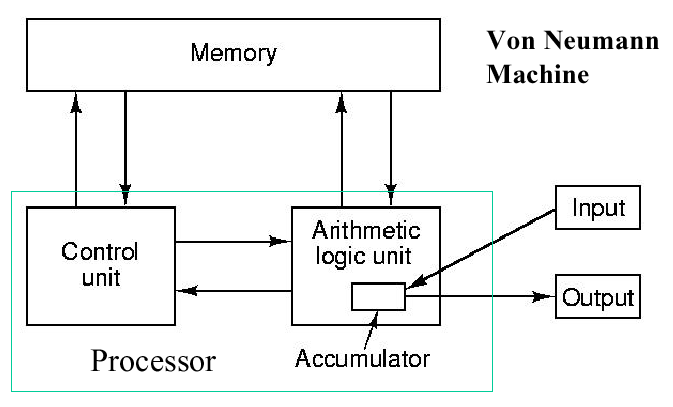
\includegraphics[width=8cm]{informatika/operacne_systemy_a_hw/obrazky/VonNeumann.png}
  \end{center}
\end{obecne}

\begin{obecne}{Harvardská}
Vytvořena až po Von Neumannově, liší se hlavně tím, že program se ukládá do jiné paměti než data (tzn. jsou 2 \uv{druhy paměti}~-- instrukcí a dat). Příklady jsou DSP procesory a mikrokontrolery (např. AVR od Atmelu, a PIC~-- mají paměť na program a data a RISC instrukční sadu; výhoda oddělených pamětí je, že můžou mít různou bitovou hloubku~-- 8 bitové data, ale 12-, 14- či 16- bitové instrukce (např. ARM musí občas použít více než jednou instrukci na zpracování obsahu plné velikosti)).

Oproti Von Neumannově nehrozí nebezpečí přepsání programu sebou samým, ale kvůli většímu počtu paměťových sběrnic je náročnější na výrobu. Paměť navíc nelze dělit podle potřeby (rozdělení je už dané).
\end{obecne}

\subsection{Procesory, multiprocesory}

\begin{definiceN}{Procesor} 
Procesor (CPU – central processing unit) je ústřední výkonnou jednotkou počítače, která čte z paměti instrukce a na jejich základě vykonává program.

Základnými súčasťami procesora sú:
\begin{pitemize}
	\item řadič nebo řídicí jednotka, která řídí tok programu, tj. načítání instrukcí, jejich dekódování, načítání operandů instrukcí z operační paměti a ukládání výsledků zpracování instrukcí
	\item sada registrů k uchování operandů a mezivýsledků.
	\item jedna nebo více aritmeticko-logických jednotek (ALU), které provádí s daty aritmetické a logické operace.
	\item některé procesory obsahují jednu nebo několik jednotek plovoucí čárky (FPU), které provádí operace v plovoucí řádové čárce.
\end{pitemize}
\end{definiceN}

\begin{poznamka}
Súčasné procesory navyše často obsahujú ďalšie rozsiahle funkčné bloky (cache, rôzne periférie)~-- ktoré z \uv{ortodoxného hladiska} nie sú priamo súčasťou \emph{jadra procesoru}. Niektoré procesory môžu obsahovať viac jadier (+logiku slúžiacu k ich vzájomnému prepojeniu). Ďalším trendom je SoC (System on Chip), kde sa na čipe procesora nachádzajú aj ďalšie subsystémy napr. na spracovanie zvuku, grafiky alebo pripojenie externých periférií (takéto riešenia sa využívajú väčšinou v PDA, domácej elektronike, mobiloch atď.).
\end{poznamka}

\begin{obecne}{Dělení podle instruční sady}
Podľa inštrukčnej sady je možné procesory rozdeliť na:
\begin{pitemize}
	\item \textbf{CISC} (Complex Instruction Set Computer): poskytuje rozsiahlu inštrukčnú sadu spolu s rôznymi variantami inštrukcií. Jedna inštrukcia napr. môže vykonať veľa low-level operácií (načítanie z pamäti, vykonať aritmetickú operáciu a výsledok uložiť). Takéto inštrukcie zjednodušovali zápis programov (inštrukcie boli bližšie vyšším programovacím jazykom) a zmenšovali veľkosť programu a počet prístupov do pamäti~-- čo bolo v 60tych rokoch dôležité. Avšak nie vždy je vykonanie jednej zložitej operácie rýchlejšie ako vykonanie viac menej zložitých miesto toho (napr. kvôli zložitému dekódovaniu a použitiu mikrokódu na volanie jednoduchých \uv{podinštrukcií}). Príkladmi CISC architektúr procesorov sú System/360, Motorola 68000 a Intel x86. V súčasnosti napr. x86 rozkladá zložité inštrukcie na \uv{micro-operations} ktoré môžu byť pipeline-ou spracované paralelne a vyšší výkon je tak dosahovaný na väčšom rozsahu inštrukcií. Vďaka tomu sú súčasné x86 procesory minimálne rovnako výkonné ako ozajstné RISC architektúry.
	\item \textbf{RISC} (Reduced Instruction Set Computer): design CPU ktorý uprednosňuje jednoduchšiu inštrukčnú sadu a menšiu zložitosť adresovacích modelov~-- vďaka čomu je možné dosiahnuť lacnejšiu implementáciu, väčšiu úroveň paralelizmu a účinnejšie kompilátory. Dôvodom vzniku bolo aj nevyužívanie celej CISC inštrukčnej sady a upredňostňovania len obmedzenej podmnožiny (designéri procesorov potom optimalizovali len tieto podmnožiny a tak sa zvyšné inštrukcie používali ešte menej...). Kvôli väčšiemu počtu inštrukcií však musia RISC procesory častejšie pristupovať k pamäti... Príkladmi RISC procesorov sú napr. SPARC a ARM. V architekturách typu \textbf{Post-RISC} jde o spojení RISCových vlastností s technikami zvýšení výkonu, jako je out-of-order vykonávání a paralelismus.
    \item \textbf{VLIW}: Very Long Instruction Word or VLIW refers to a CPU architecture designed to take advantage of instruction level parallelism (ILP). A processor that executes every instruction one after the other (i.e. a non-pipelined scalar architecture) may use processor resources inefficiently, potentially leading to poor performance. The performance can be improved by executing different sub-steps of sequential instructions simultaneously (this is pipelining), or even executing multiple instructions entirely simultaneously as in superscalar architectures. The VLIW approach, on the other hand, executes operation in parallel based on a fixed schedule determined when programs are compiled. Since determining the order of execution of operations (including which operations can execute simultaneously) is handled by the compiler, the processor does not need the scheduling hardware that the three techniques described above require. As a result, VLIW CPUs offer significant computational power with less hardware complexity (but greater compiler complexity) than is associated with most superscalar CPUs.
    \item \textbf{EPIC}: (Někdy označován za poddruh VLIW) Explicitly Parallel Instruction Computing (EPIC) is a computing paradigm that began to be researched in the 1990s. This paradigm is also called Independence architectures. It was used by Intel and HP in the development of Intel’s IA-64 architecture, and has been implemented in Intel’s Itanium and Itanium 2 line of server processors. The goal of EPIC was to increase the ability of microprocessors to execute software instructions in parallel, by using the compiler, rather than complex on-die circuitry, to identify and leverage opportunities for parallel execution. This would allow performance to be scaled more rapidly in future processor designs, without resorting to ever-higher clock frequencies, which have since become problematic due to associated power and cooling issues.
\end{pitemize}
\medskip
TODO: asi opravit, možná zpřesnit VLIW a EPIC a určitě přeložit

\medskip
Řekneme, že procesor má \emph{ortogonální instrukční sadu}, pokud žádná instrukce nepředpokládá implicitně použití některých registrů. To umožňuje jednodušší práci algoritmům přidělování registrů v překladačích. Příkladem neortogonální instrukční sady je i x86.
\end{obecne}

\begin{obecne}{Další dělení}
Ďalej je možné procesory rozdeliť podľa dĺžky operandov v bitoch (8, 16, 32, 64...), ktorý je procesor schopný spracovať v jednom kroku. V embedded zariadeniach sa najčastejšie používajú 4- a 8-bitové procesory. V PDA, mobiloch a videohrách 8 resp. 16 bitové. 32 a viac bitov využíajú napr. osobné počítače a laserové tlačiarne.

Dôležitou vlastnosťou je aj taktovacia frekvencia jadra, MIPS (millions of instructions per second) a jeho rýchlosť. V súčasnosti je ťažké dávať do súvislosti výkon procesorov s ich frekvenciou (resp. MIPS)~-- kým Pentium zvládne na výpočet vo floatoch, jednoduchý 8-bitový PIC na to potrebuje oveľa viac taktov. Ďalším \uv{problémom} je superskalarita procesorov, ktorá im umožňuje vykonať viacero nezávislých inštrukcií počas jedného taktu.
\end{obecne}

\begin{obecne}{Techniky pro zvýšení výkonu}
Zvyšovať výkon (procesorov) je možné viacerými spôsobmi. Najjednoduchším (a najpomalším) typom je Subskalárny CPU (načíta a spracúva len jednu inštrukciu naraz~-- preto musí celý procesor čakať kým vykonávanie inštrukcie skončí; je tak zdržovaný dlhšie trvajúcimi inštrukciami). 

\begin{center}
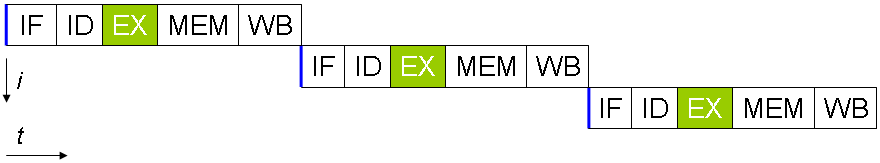
\includegraphics[width=8cm]{informatika/operacne_systemy_a_hw/obrazky/Nopipeline.png}
\end{center}

Pokusy o dosiahnutie skalárneho a lepšieho výkonu vyústili do designov ktoré sa správajú menej lineárne a viac paralelne. Čo sa týka paralelizmu v procesoroch, používajú sa dva druhy pojmov na ich klasifikáciu~-- \emph{Instruction level parallelism} (zvyšovanie rýchlosti vykonávania inštrukcií v procesore a teda zväčšovanie využitia prostriedkov na čipe) a \emph{Thread level parallelism} (zväčšovanie počtu vlákien, ktoré dokáže CPU vykonávať naraz).
\begin{pitemize}
  \item \textbf{pipeline}: 
  Zlepšenie je možné dosiahnúť pomocou \uv{instruction pipelining}-u, ktoré je použíté vo väčšine moderných procesorov. Umožňuje vykonanie viac ako jednej inštrukcie v jednom kroku vďaka rozloženiu spracovávania inštrukcie na viac menších krokov: 
  \begin{center}
  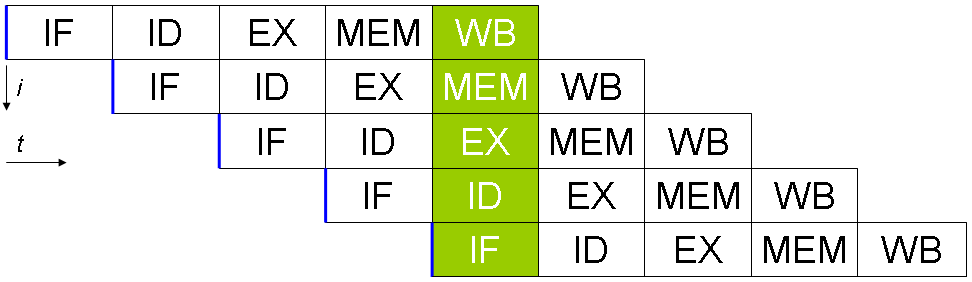
\includegraphics[width=8cm]{informatika/operacne_systemy_a_hw/obrazky/Fivestagespipeline.png}
  \end{center}

  \item \textbf{superskalarita}: Dialša možnosť je použitie superscalar designu, ktorý obsahuje dlhú inštrukčnú pipeline a viacero identických execution jednotiek.  
  \begin{center}
  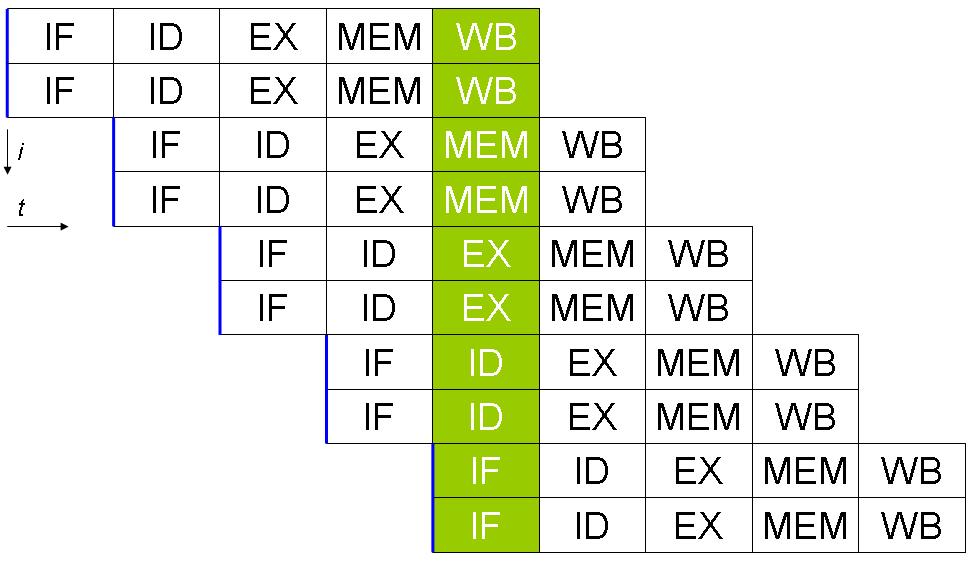
\includegraphics[width=8cm]{informatika/operacne_systemy_a_hw/obrazky/Superscalarpipeline.png}
  \end{center}	

  \item \textbf{Out of order execution}
  \begin{penumerate}
	  \item Načtení instrukce, případně její rozdrobení na mikroinstrukce
	  \item Zařazení do vyčkávací stanice (instruction pool)
	  \item Instrukce čeká na všechny svoje operandy
	  \item Instrukce se vykoná ve své výkonné jednotce (je vybírána z instruction poolu nezávisle na ostatních)
	  \item Výsledky se uchovají ve frontě (reorder buffer)
	  \item Až se všechny starší instrukce zapíší do registrů, zapíše se výsledek této instrukce (opětovné řazení)
  \end{penumerate}

  \item \textbf{Predikce skoků}~-- hluboké pipeliny mají problém, pokud podmíněný skok není proveden; dynamická predicke skoků (historie CPU~-- vzory nějaké hloubky) vs. statická (bez nápovědy~-- skok vpřed se neprovede, skok vzad se provede; s nápovědou~-- překladač odhaduje pravděpodobnost skoku)

  \item \textbf{Spekulativní vykonávaní}~-- vykonávání kódu, který nemusí být zapotřebí; významná disproporce mezi rychlostí CPU a paměti; typické využití je značné předsunutí čtecích operací; CPU provádí i odsouvání zápisových operací


  \item \textbf{Data parallelism}: SIMD inštrukcie (napr. multimediálne inštrukcie), vektorové procesory...
\end{pitemize}
\end{obecne}

\subsubsection*{Multiprocesory}

TODO: jde o copy \& paste z Wiki ... předělat česky/slovensky
\medskip

\begin{definiceN}{Multiprocesor}
  O \emph{multiprocesoru} mluvíme, pokud je použito dvou nebo více procesorů
  (CPU) v rámci jednoho počítačového systému. Termín je také používán mluvíme-li
  o schopnosti systému využívat více procesorů a/nebo schopnosti rozdělovat
  úlohy mezi jednotlivými procesory.
\end{definiceN}

\begin{obecne}{Vztah k datům a instrukcím}
In multiprocessing, the processors can be used to execute a single sequence of instructions in multiple contexts (single-instruction, multiple-data or SIMD, often used in vector processing), multiple sequences of instructions in a single context (multiple-instruction, single-data or MISD, used for redundancy in fail-safe systems and sometimes applied to describe pipelined processors or hyperthreading), or multiple sequences of instructions in multiple contexts (multiple-instruction, multiple-data or MIMD).
\end{obecne}

\begin{obecne}{Symetrie}
In a multiprocessing system, all CPUs may be equal, or some may be reserved for special purposes. A combination of hardware and operating-system software design considerations determine the symmetry (or lack thereof) in a given system. For example, hardware or software considerations may require that only one CPU respond to all hardware interrupts, whereas all other work in the system may be distributed equally among CPUs; or execution of kernel-mode code may be restricted to only one processor (either a specific processor, or only one processor at a time), whereas user-mode code may be executed in any combination of processors. Multiprocessing systems are often easier to design if such restrictions are imposed, but they tend to be less efficient than systems in which all CPUs are utilized equally.

Systems that treat all CPUs equally are called symmetric multiprocessing (SMP) systems. In systems where all CPUs are not equal, system resources may be divided in a number of ways, including asymmetric multiprocessing (ASMP), non-uniform memory access (NUMA) multiprocessing, and clustered multiprocessing (qq.v.).
\end{obecne}

\begin{obecne}{Těsnost spojení multiprocesorů}
\begin{pitemize}
    \item \textbf{Tightly-coupled} multiprocessor systems contain multiple CPUs that are connected at the bus level. These CPUs may have access to a central shared memory (SMP or UMA), or may participate in a memory hierarchy with both local and shared memory (NUMA). The IBM p690 Regatta is an example of a high end SMP system. Intel Xeon processors dominated the multiprocessor market for business PCs and were the only x86 option till the release of AMD's Opteron range of processors in 2004. Both ranges of processors had their own onboard cache but provided access to shared memory; the Xeon processors via a common pipe and the Opteron processors via independent pathways to the system RAM.

    \item \textbf{Chip multiprocessors}, also known as multi-core computing, involves more than one processor placed on a single chip and can be thought of the most extreme form of tightly-coupled multiprocessing. Mainframe systems with multiple processors are often tightly-coupled.

    \item \textbf{Loosely-coupled multiprocessor} systems (often referred to as clusters) are based on multiple standalone single or dual processor commodity computers interconnected via a high speed communication system (Gigabit Ethernet is common). A Linux Beowulf cluster is an example of a loosely-coupled system.
\end{pitemize}
Tightly-coupled systems perform better and are physically smaller than loosely-coupled systems, but have historically required greater initial investments and may depreciate rapidly; nodes in a loosely-coupled system are usually inexpensive commodity computers and can be recycled as independent machines upon retirement from the cluster.

\textbf{SMP} (Symmetric Multiprocessing): viac procesorov so zdieľanou operačnou pamäťou (nutné mechanizmy na zabránenie nesprávnych náhľadov na pamäť a migráciu procesov medzi procesormi). SMP systems allow any processor to work on any task no matter where the data for that task are located in memory; with proper operating system support, SMP systems can easily move tasks between processors to balance the workload efficiently.
\end{obecne}

\subsection{Sběrnice, protokoly}

\begin{pitemize}
	\item \textbf{Struktura sběrnice}: datové linky, adresové linky, řídící linky
	\item \textbf{Synchronní přenos} (vznik události je dán hodinovým signálem) vs. \textbf{asynchronní přenos} (vznik události je určen předcházející událostí~-- napr. signalizáciou začiatku dát) 
	\item \textbf{Parametry sběrnice}: 
	\begin{pitemize}
	  \item \emph{datová šířka}~-- počet přenášených bitů v jednom okamžiku,
	  \item \emph{kapacita}~-- počet bitů přenesených za čas,
	  \item \emph{rychlost}~-- kapacita sběrnice normovaná k jednotce informace. 
	\end{pitemize}  
	\item \textbf{Řízení požadavků}: 
	\begin{pitemize}
	  \item \emph{centrální}~-- náhodné, dle pořadí vzniku požadavků, prioritní,
	  \item \emph{distribuované}~-- kolizní (CSMA/CD), token bus, prioritní linka (daisy chain).
	\end{pitemize} 
	\item \textbf{Přenos dat po sběrnici} může probíhat buď za účasti procesoru (zdroj $\rightarrow$ CPU $\rightarrow$ cíl), nebo bez. Bez procesoru to může být např.:
	\begin{pitemize}
		\item dávkový režim~-- domluva mezi CPU a řadičem na době obsazení sběrnice (napr. pomocou zdvihnutia \uv{lock flagu} na zbernici)
		\item kradení cyklů~-- řadič na dobu přenosu \uv{uspí} procesor (nelze uspat na dlouho, je to technicky náročnější)
		\item transparentní režim~-- řadič rozezná, kdy procesor nepoužívá sběrnici, obvykle nelze větší přenosy najednou
		\item DMA (Direct Memory Access)~-- speciální jednotka pro provádění přenosů dat (mezi zařízeními a pamětí)
	\end{pitemize}
	Jednou z technik, používaných k přenosu dat po sběrnici řadiči DMA, je \emph{scatter-gather}. Znamená to, že v rámci jednoho přenosu se zpracovává víc ne nutně souvislých bloků dat. 
	\begin{pitemize}
	    \item \emph{scatter}~-- DMA řadič v rámci 1 přenosu uloží z 1 místa data na několik různých míst (např hlavičky TCP/IP - jinak zbytečné kopírování)  
	    \item \emph{gather}~-- např. při stránkování paměti - načítání stránek, které fyzicky na disku nemusí být u sebe, složení na 1 místo do paměti.
	\end{pitemize}
\end{pitemize}

Příklady sběrnic:
\begin{pitemize}
	\item ISA, EISA
	\item ATA, ATAPI~-- UltraDMA, Serial-ATA (SATA)
	\item SCSI (Small Computer System Interface)
	\item PCI, PCI-X, PCI Express
	\item AGP (Advanced Graphics Port)
	\item USB (Universal Serial Bus)
	\item FireWire (IEEE 1394)
	\item RS485
	\item $I^{2}C$
\end{pitemize}

Příbuzné sběrnic:
\begin{pitemize}
	\item IrDA
	\item Bluetooth
	\item Wi-Fi, WiMAX 
\end{pitemize}

\subsection{Vstupní a výstupní zařízení}

K I/O zařízením je možné přistupovat dvěma způsoby: pomocí \textbf{port}ů (speciální adresový port CPU) nebo \textbf{pamětovým mapováním} (namapování do fyzické paměti).

Zařízení mají různé charakteristiky:
\begin{pitemize}
	\item \textbf{druh}~-- blokové (disk, síťová karta), znakové (klávesnice, myš)
	\item \textbf{přístup}~-- sekvenční (datová páska), náhodný (hdd, cd)
	\item \textbf{komunikace}~-- synchronní (pracuje s daty na žádost~-- disk), asynchronní (\uv{nevyžádaná} data~-- síťová karta)
	\item \textbf{sdílení}~-- sdílené (preemptivní, lze odebrat~-- síťová karta (po multiplexu OS)), vyhrazené (nepreemptivní~-- tiskárna, sdílení se realizuje přes \emph{spooling}). Reálně se rozdíly stírají.
	\item \textbf{rychlost} (od několika Bps po GBps)
	\item \textbf{směr dat}~-- R/W, R/O (CD-ROM), W/O (tiskárna) 
\end{pitemize}

Přenos dat mezi zařízením a CPU/pamětí:
\begin{pitemize}
	\item \textbf{polling}~-- aktivní čekání na změnu zařízení, přenos provádí CPU
	\item \textbf{přerušení}~-- asynchronní přerušení od zařízení, přenos provádí CPU
	\item \textbf{DMA (Direct Memory Access)}~-- zařízení si samo řídí přístup na sběrnici a přenáší data z/do paměti; po skončení přenosu přerušení (oznámení o dokončení)
\end{pitemize}

Cíle I/O software:
\begin{pitemize}
	\item \textbf{Nezávislost zařízení}~-- programy nemusí dopředu vědět, s jakým přesně zařízením budou pracovat~-- je jedno jestli pracuji se souborem na pevném disku, disketě nebo na CD-ROM
	\item \textbf{Jednotné pojmenování} (na UNIXu /dev)
	\item \textbf{Připojení (mount)}~-- časté u vyměnitelných zařízení (disketa); možné i u pevných zařízení (disk); nutné pro správnou funkci cache OS
	\item \textbf{Obsluha chyb}~-- v mnoha případech oprava bez vědomí uživatele (velmi často způsobeno právě uživatelem)
\end{pitemize}

\subsection{Architektury OS}

\begin{obecne}{Klasická struktura~-- monolitická}
Nejstarší, už IBM 360, Unix, Win., všechny služby uvnitř, prováděny ve chráněném módu, jádro poměrně velké, \uv{údajně} nejrychlejší. Program zavolá službu OS, přes tabulku se zjistí adresa přísl. fce, ta se zavolá a vrátí výsledek.  Nevýhoda: horší údržba -- je-li v programu chyba, může poškodit zbývající části systému, rozšiřování za běhu je komplikované. 
\end{obecne}

\begin{obecne}{Virtuální stroje}
Původní nápad : Virtual Machine pro IBM360 -- oddělit multitasking od OS jako ext. stroj. Nad HW byla další vrstva -- \uv{Virtual Machine} -- měla plánovat, vyrábí pro procesy iluzi holého HW; dneska např. VMWare dělá to samé. Pro IBM360 se dalo použít v kombinaci s CMS (jednoúlohový) i původního OS360 (rychlejší než OS360 na holém HW). 

Dnes: definuji abstraktní stroj, pro něj překládám programy (.NET, Java) $\rightarrow$ přenositelnost, kompatibilita (IBM AS400~-- desítky let), problém~-- pomalé. 
\end{obecne}

\begin{obecne}{Mikrojádro}
snaha aby část běžící v kernel módu byla co nejmenší (třeba jen cca 10 KB), nejnovější, experimentální, často pro Distribuované OS (dnes už nepoužívané), hodně procesů \& komunikace (klient/server), mikrojádro řeší jenom komunikaci. 

Filesystém apod. jsou procesy -- aplikace jim posílají přes jádro požadavky. Jediný komerční OS -- Chorus (ústředny). výhoda: když něco spadne, nepoškodí to zbytek, moduly jdou měnit za běhu, komunikace jde snadno rozšířit na komunikaci po síti. 
\end{obecne}

\begin{obecne}{Architektura WinNT}
  Jádro je poměrně malé (cca 1MB), schopné (pro vyšší vrstvy jsou některé schopnosti skryté), na jeho vzniku se podíleli schopní Unixáři. Byla zde snaha o malou velikost, přenositelnost. Jádro je neutrální vzhledem k vyšším vrstvám, nad ním lze vybudovat různé systémy (Windows subsystém, POSIX, OS/2).

  Rozhraní OS a uživ. programů zajišťuje WinAPI, nad ním se nacházejí různé DLL, mezi kernelem a HW je \uv{hardware abstraction layer}, tj. kernel lze jednoduše upravit pro jiné architektury (Alpha, IA-64).
  Grafické drivery jediné mají přímý přístup k HW (kvůli výkonu), části API (USER, GDI) jsou implementované v jádře, přechod mezi user a kernel režimem zajišťuje ntdll.dll (a je tedy využíván všemi programy). Veškeré služby a aplikace běží v user módu nad jádrem.

  \begin{center}
    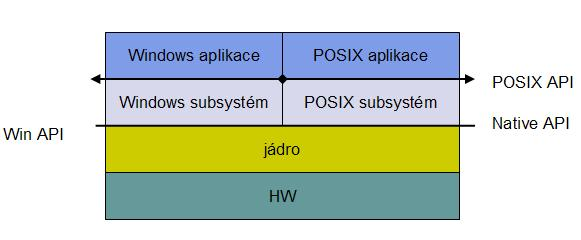
\includegraphics[width=8cm]{informatika/operacne_systemy_a_hw/obrazky/arch-windows.jpg}
  \end{center}
\end{obecne}

\begin{obecne}{Architektura Linuxu}
  \begin{pitemize}
      \item Na úrovni SW -- přenositelnost; abstrakce HW. 
      \item nad HW~-- kernel, nad ním systémová volání, hodně podobné Windows.
  \end{pitemize}

  \begin{center}
    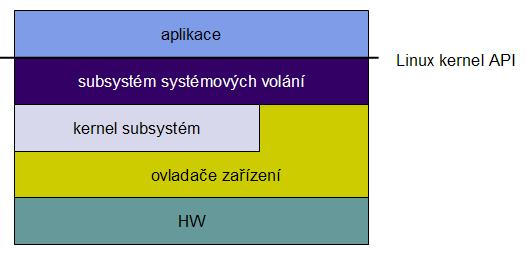
\includegraphics[width=8cm]{informatika/operacne_systemy_a_hw/obrazky/arch-linux.jpg}
  \end{center}
\end{obecne}

\subsection{Vztah OS a HW, obsluha přerušení}

\begin{obecne}{Zjištění změny stavu I/O zařízení:}
\begin{pitemize}
	\item \emph{asynchronní přerušení}~-- zašle zařízení
	\item \emph{polling}~-- peridická kontrola stavu zařízení
\end{pitemize}
\end{obecne}

\begin{obecne}{Druhy přerušení:}
\begin{pitemize}
	\item \emph{synchronní}~-- záměrně (instrukce TRAP~-- vstup do OS), výjimky (nesprávné chování procesu)~-- zpracuje se okamžitě
	\item \emph{asynchronní}~-- vnější událost (např. příchod dat)~-- zpracuje se po dokončení aktuální instrukce 
\end{pitemize}
\end{obecne}

\begin{obecne}{Obsluha přerušení:}
\begin{pitemize}
	\item OS se ujme řízení
	\item uloží se stav CPU (obsah registrů, čítač, ...)
	\item analyzuje se přerušení, vyvolá se příslušná obsluha (pokud není přerušení blokováno)
	\item obslouží se přerušení (např. se zavolá obslužná procedura)
	\item obnoví se stav CPU a aplikace pokračuje, popř. může dojít k přeplánování 
\end{pitemize}
\end{obecne}

\begin{obecne}{I/O software (vrstvy):}
\begin{pitemize}
	\item uživatelský I/O software
	\item I/O nezávislý subsystém
	\item ovladače zařízení
	\item obsluha přerušení 
\end{pitemize}
\end{obecne}

\begin{obecne}{Cíle I/O software:}
\begin{pitemize}
	\item nezávislost zařízení~-- programy nemusí vědět, s jakým přesně pracují
	\item jednotné pojmenování (/dev)
	\item připojení (mount)~-- vyměnitelná zařízení
	\item obsluha chyb
\end{pitemize}
\end{obecne}

\subsection{Procesy, vlákna, plánování}

\subsubsection*{Procesy a vlákna}
Systémové volání je interface mezi OS (kernelspace) a užívatelskými programy (userspace).

\begin{definiceN}{Proces}
  \emph{Proces} je inštancia vykonávaného programu. Kým program je len súbor
  inštrukcií, proces je vlastný \uv{výkon} týchto inštrukcií. Proces má vlastný
  adresný priestor (pamäť), prostriedky, práva a napr. aj ID (Process ID).
\end{definiceN}

Počas života sa môže proces nachádzať v rôznych stavoch:
\begin{pitemize}
  \item \emph{bežiaci}~-- jeden proces na procesor,
  \item \emph{blokovaný}~-- pri použití blokujúceho volania~-- I/O disku atď.,
  \item \emph{pripravený}~-- skončilo blokovanie; spotreboval všetok pridelený čas resp. vrátil riadenie systému, čaká na nové pridelenie procesora,
  \item \emph{zombie}~-- po ukončení procesu, keď už nepracuje~-- ale ešte nebol vymazaný.
\end{pitemize}

\begin{definiceN}{Vlákno}
  \emph{Vlákno} je možnosť pre program ako sa \uv{rozdeliť} na dva alebo viac
  zároveň (resp. pseudo-zároveň) vykonávaných úloh. Oproti procesu mu nie je
  pridelená vlastná pamäť~-- je to len miesto vykonávania inštrukcií v programe.
  Oproti procesu sú jeho \uv{atribútmi} len hodnota programového čítača, stav
  registrov CPU a zásobník.
\end{definiceN}

Oproti Windows/Solaris neobsahuje Linux priamu podporu pre vlákna. Miesto toho podporuje procesy (zhodou okolností :-)) zdieľajúce pamäť. V samotnom jadre linuxu ale vlákna existujú (kthreads).

\subsubsection*{Plánovanie}

Prideľovanie procesorového času jednotlivým procesom má na starosti \emph{plánovač}. Plánovanie pritom môže byť preemptívne alebo nepreemptívne (kooperatívne~-- alla Win16).

\begin{obecne}{Ciele plánovania (niektoré z nich sú očividne protichodné):}
\begin{pitemize}
	\item Spravodlivosť (každy procesor dostane adekvátnu časť času CPU)
	\item Efektívnosť (plne vyťažený procesor)
	\item Minimálna doba odpovede
	\item Průchodnost (maximálny počet spracovaných procesov)
	\item Minimálna réžia systému
\end{pitemize}
\end{obecne}

\begin{obecne}{Kritériá plánovania:}
\begin{pitemize}
	\item Viazanosť procesu na dané CPU a I/O (presun procesu na iný procesor zaberie veľa prostriedkov)
	\item Proces je dávkovy/interaktívny?
	\item Priorita procesu (statická (nemenná~-- okrem \uv{renice}) + dynamická, ktorá sa mení v čase kvôli spravodlivosti)
	\item Ako často proces generuje výpadky stránok (nejaký popis???)
	\item Kolik skutočného času CPU proces obdržel
\end{pitemize}
\end{obecne}

\begin{obecne}{Algoritmy:}
\begin{pitemize}
	\item \textbf{FIFO}: nepreemptívny, proces opustí procesor až po skončení

	\item \textbf{Round Robin}: preemptívne rozšírenie FIFO, po skončení časového kvanta je proces presunutý na koniec fronty

	\item \textbf{Plánovanie s viacerými frontami}: niekoľko front, procesu z $i$-tej fronty je pridelený procesor až keď vo frontách $1, \dots, i-1$ nie je pripravený ziadny proces. Ak proces skončil I/O operáciou, je blokovaný a presunutý do fronty $i-1$, ak skončil preempciou, je pripravený a presunutý do fronty $i+1$.

	\item \textbf{SMP}: fronta CPU čakajúcich na pripravené procesy (aktívne (spotrebováva energiu) vs. pasívne čakanie (špeciálne inštrukcie)), \uv{vzťah}/afinita procesov k CPU

	\item TODO: Plánovanie windows vs. linux???
\end{pitemize}
\end{obecne}

\subsection{Synchronizační primitiva, vzájemné vyloučení}

\subsubsection*{Pojmy}

\emph{Race conditions}: výsledek operace závisí na plánování

\emph{Vzájemné vyloučení (mutual exclusion)}: kritickou operaci provádí nejvýše jeden proces. Podmínky vzájemného vyloučení:
\begin{penumerate}
	\item Žádné dva procesy nemohou být najednou ve stejné kritické sekci
	\item Nemohou být učiněny žádné předpoklady o rychlosti nebo počtu CPU
	\item Žádný proces mimo kritickou sekci nesmí blokovat jiný proces
	\item Žádný proces nesmí čekat nekonečně dlouho v kritické sekci
\end{penumerate}

\emph{Kritická sekce}: část programu, kde se provádí kritická operace

Metody dosáhnutí vzájemného vyloučení: aktivní čekání (busy waiting) a pasivní čekání/blokování.

\subsubsection*{Aktivní čekání}
\emph{Vlastnosti}: spotřebovává čas procesoru, vhodnější pro předpokládané krátké doby čekání, nespotřebovává prostředky OS, rychlejší.

Je možné použít např. \emph{zakázání přerušení} (vhodné pro jádro OS). Používání \emph{zámků} nefunguje:
\begin{verbatim}
int lock;
void proc(void) {
  for (;;) {
    nekritická_sekce();
    while (lock != 0);
    lock = 1;
    kritická_sekce();
    lock = 0;
  }
}
\end{verbatim}
ale \emph{důsledné střídání} ano (to ale porušuje podmínku 3.)

\begin{verbatim}
int turn = 0;

void p1(void)                void p2(void)
{                            {
  for (;;) {                   for (;;) {
    while (turn != 0);           while (turn != 1);
    kritická_sekce();            kritická_sekce();
    turn = 1;                    turn = 0;
    nekritická_sekce();          nekritická_sekce();
  }                            }
}                            }
\end{verbatim}

\emph{Petersonovo řešení}:
\begin{verbatim}
#define N 2                   /* počet procesů */
 
int turn;
int interested[N];            /* kdo má zájem */
 
void enter_region(int proc) { /* proc: kdo vstupuje */
int other;
 
  other = 1-proc;             /* číslo opačného procesu */
  interested[proc] = TRUE;    /* mám zájem o vstup */
  turn = proc;                /* nastav příznak */
  while (turn == proc && interested[other] == TRUE);
}
 
void leave_region(int proc) { /* proc: kdo vystupuje */
  interested[proc] = FALSE;   /* už odcházím */
}
\end{verbatim}
 
\emph{Instrukce TSL} (spin-lock) - je nutné aby ji podporoval HW (všechny současné procesory nějakou mají):
\begin{verbatim}
enter_region:
    tsl   R,lock           ; načti zámek do registru R a
                           ; nastav zámek na 1
    cmp   R,#0             ; byl zámek nulový?
    jnz   enter_region     ; byl-li nenulový, znova
    ret                    ; návrat k volajícímu - vstup do
                           ; kritické sekce
 leave_region:
    mov   lock,#0          ; ulož do zámku 0
    ret                    ; návrat k volajícímu
\end{verbatim}

\subsubsection*{Pasivní čekání}
\emph{Vlastnosti}: proces je ve stavu blokován, vhodné pro delší doby čekání, spotřebovává prostředky OS, pomalejší.

Postup používající Sleep/Wakeup (implementovány OS, atomické operace - sleep uspí volající proces, wakeup probudí udaný proces) nefunguje (viď Problém producent/konzument).

\textbf{Semafory}... Sémantika:
\begin{verbatim}
Down(Semaphore s) {
  wait until s > 0, then s := s-1;
  /* must be atomic once s > 0 is detected */
}
\end{verbatim}
(pokud je čítač $>$ 0, sníží čítač o 1 a pokračuje dál; pokud je čítač $=$ 0, operace DOWN se zablokuje a proces je přidán do fronty čekající na tomto semaforu)

\begin{verbatim}
Up(Semaphore s) {
  s := s+1;   /* must be atomic */
}
\end{verbatim}
(pokud je fronta neprázdná, vybere libovolný proces a ten probudí za DOWN; jinak zvětší čítač o 1)

\begin{verbatim}
Init(Semaphore s, Integer v) {
  s := v;
}
\end{verbatim}

Je možné \uv{používať} aj sémantiku, kde sa hodnota vždy zníži/zvýši o 1 (a je možné sa teda dostať do záporných hodnôt semafóru)... Špeciálny (binárny) typ semaforu, kde sú povolené len hodnoty 0 a 1 (v Up sa miesto $s:=s+1$ volá $s:=1$) sa nazýva \emph{mutex} a používa sa na riadenie prístupu k jednej premennej.

\textbf{Monitory}
\par Implementovány překladačem, lze si představit jako třídu C++ (všechny proměnné privátní, funkce mohou být i veřejné), vzájemné vyloučení v jedné instanci (zajištěno synchronizací na vstupu a výstupu do/z veřejných funkcí, synchronizace implementována blokovacím primitivem OS). ???TODO

\textbf{Zprávy}
\par Operace SEND a RECEIVE, zablokování odesílatele/příjemce, adresace proces/mailbox, rendez-vous...

\textbf{RWL - read-write lock}, \textbf{bariéry}...

Ekvivalence primitiv - pomocí jednoho blokovacího primitiva lze implementovat jiné blokovací primitivum.

Rozdíly mezi platformami: Windows - jednotné funkce pro pasivní čekání, čekání na více primitiv, timeouty. Unix - OS implementuje semafor, knihovna pthread.

\subsubsection*{Klasické synchronizační problémy}
\textbf{Problém producent/konzument}
\par Producent vyrába predmety, konzument ich spotrebúva. Medzi nimi je sklad pevnej veľkosti (N). Konzument nemá čo spotrebúvať ak je sklad prázdny; producent prestane vyrábať, ak je sklad plný. 

\begin{verbatim}
int N = 100;
int count = 0;
void producer(void) {
    int item;
    while(TRUE) {
        produce_item(&item);
        if(count==N) sleep ();
        enter_item(item);
        count++;
        if(count == 1) wake(consumer);
    }
}
void consumer(void) {
    int item;
    while(TRUE) {
        if(count==0) sleep ();
        remove_item(&item);
        count--;
        if(count==N-1)
            wake(producer);
        consume_item(&item);
    }
}
\end{verbatim}

\begin{penumerate}
	\item Buffer je prázdny, a konzument práve prečítal count, aby zistil, či je rovný nule
	\item Preplánovanie na producenta
	\item Producent vytvorí item a zvýši count
	\item Producent zistí, či je count rovný jednej. Zistí že áno, čo znamená že konzument bol predtým zablokovaný (pretože muselo byť 0), a zavolá wakeup
	\item Teraz môže dôjsť k zablokovaniu: konzument sa uspí, pretože si myslí, že nemá čo zobrať; producent bude chvíľu produkovať a dôjde "preplneniu" $\Rightarrow$ uspí sa; spí producent aj konzument :o) 
\end{penumerate}

\textbf{Problém obědvajících filosofů}
\par Pět filosofů sedí okolo kulatého stolu. Každý filosof má před sebou talíř špaget a jednu vidličku. Špagety jsou bohužel slizké a je třeba je jíst dvěma vidličkami. Život filosofa sestává z období jídla a období přemýšlení. Když dostane hlad, pokusí se vzít dvě vidličky, když se mu to podaří, nají se a vidličky odloží.

\textbf{Problém ospalého holiče}
\par Holič má ve své oficíně křeslo na holení zákazníka a pevný počet sedaček pro čekající zákazníky. Pokud v oficíně nikdo není, holič se posadí a spí. Pokud přijde první zákazník a holič spí, probudí se a posadí si zákazníka do křesla. Pokud přijde zákazník a holič už střihá a je volné místo v čekárně, posadí se, jinak odejde.

\subsection{Zablokování a zotavení z něj}

Prostředek je cokoliv, k čemu je potřeba hlídat přístup (HW zařízení~-- tiskárny, cpu; informace~-- záznamy v DB). Je možné je rozdělit na \emph{odnímatelné} (lze odejmout procesu bez následků~-- CPU, paměť) a \emph{neodnímatelné} (nelze odejmnout bez nebezpečí selhání výpočtu~-- CD-ROM, tiskárna... tento druh způsobuje problémy).

Práce s prostředky probíhá v několika krocích: \emph{žádost o prostředek} (blokující, právě tady dochází k zablokování), \emph{používání} (např. tisk), \emph{odevzdání} (dobrovolné/při skončení procesu).

Množina procesů je \emph{zablokována}, jestliže každý proces z této množiny čeká na událost, kterou může způsobit pouze jiný proces z této množiny.

\subsubsection*{Coffmanovy podmínky}
Splnenie týchto podmienok je nutné pre zablokovanie:
\begin{penumerate}
	\item \textbf{Vzájemné vyloučení} – každý prostředek je buď vlastněn právě jedním procesem nebo je volný.
	\item \textbf{Drž a čekej} – procesy aktuálně vlastnící nějaké prostředky mohou žádat o další.
	\item \textbf{Neodnímatelnost} – přidělené prostředky nemohou být procesům odebrány.
	\item \textbf{Čekání do kruhu} – existuje kruhový řetěz procesů, kde každý z nich čeká na prostředek vlastněný dalším článkem řetězu.
\end{penumerate}

\subsubsection*{Řešení zablokování}
\begin{pitemize}
	\item \textbf{Pštrosí algoritmus}~-- Zablokování se ani nedetekuje, ani se mu nezabraňuje, ani se neodstraňuje, Uživatel sám rozhodne o řešení (kill). Nespotřebovává prostředky OS~-- nemá režii ani neomezuje podmínky provozu. (Nejčastější řešení~-- Unix, Windows) 
	\item \textbf{Detekce a zotavení}~-- Hledá kružnici v orientovaném grafu (hrany vedou od procesu, který čeká, k procesu, který prostředek vlastní), pokud tam je kružnice, nastalo zablokování a je třeba ho řešit:
		\begin{pitemize}
			\item \emph{Odebrání prostředku}~-- dohled operátora, pouze na přechodnou dobu
			\item \emph{Zabíjení procesů z cyklu} (resp. mimo cyklus vlastnící identický prostředek)
			\item \emph{Rollback} (OS ukládá stav procesů, při zablokování se některé procesy vrátí do předchozího stavu $\Rightarrow$ ztracena práce... obdoba u DB)
		\end{pitemize}
	\item \textbf{Vyhýbání se}~-- Bezpečný stav (procesy/prostředky nejsou zablokovány, existuje cesta, jak uspokojit všechny požadavky na prostředky spouštěním procesů v jistém pořadí); Viď. bankéřův algoritmus. Nutné je předem znát všechny prostředky, které budou programy potřebovat; OS pak dává prostředky tomu, který je nejblíž svému maximu potřeby a navíc pro který je prostředků dost na dokončení. Dnes se moc nepoužívá.
	\item \textbf{Předcházení (prevence)}~-- napadení jedné z Coffmanovy podmínek
		\begin{penumerate}
			\item \emph{Vzájemné vyloučení}~-- \emph{spooling} (prostriedky spravuje jeden systemový proces, ktory dohliada na to, aby jeho stav bol konzistentny (tiskarna)~-- pozor na místo na disku)
			\item \emph{Drž a čekej}~-- žádat o všechny prostředky před startem procesu. Nejprve všechno uvolnit a pak znovu žádat o všechny najednou
			\item \emph{Neodnímatelnost}~-- vede k chaosu
			\item \emph{Čekání do kruhu}~-- nejvýše jeden prostředek~-- všechny prostředky jednoznačně očíslovány, procesy mohou žádat o prostředky jen ve vzestupném pořadí

		\end{penumerate}
			\item \emph{Dvojfázové zamykání}~-- nejprve postupně všechno zamykám (první fáze). Potom se může pracovat se zamčenými prostředky~-- a na závěr se už jen odemyká (druhá fáze)~-- viď transakční spracování u databází ((striktní/konzervativní) dvoufázové zpracování)
\end{pitemize}

\textbf{Bankéřův algoritmus}: Bankéř má klienty a těm slíbil jistou výšku úvěru. Bankéř ví, že ne všichni klienti potřebují plnou výši úvěru najednou. Klienti občas navštíví banku a žádají postupně o prostředky do maximální výšky úvěru. Až klient skončí s obchodem, vrátí bance vypůjčené peníze. Bankéř peníze půjčí pouze tehdy, zůstane-li banka v bezpečném stavu.

\subsection{Organizace paměti, alokační algoritmy}

\textbf{Hierarchie paměti} (směrem odshora dolů roste velikost, cena na bajt a rychlost klesá~-- a naopak\dots):
\begin{pitemize}
    \item \emph{registry CPU} --- 10ky-100vky bajtů (IA-32: obecné registy pár 10tek), IA-64~-- až kB (extrém), stejně rychlé jako CPU. 
    \item \emph{cache} --- z pohledu aplikací není přímo adresovatelná; dnes řádově MB, rozdělení podle účelu, několik vrstev. L1 cache (cca 10ky kB)~-- dělené instrukce/data; L2 (cca MB) sdílené instr\&data, běží na rychlosti CPU (dřív bývala pomalejší), servery~-- L3 (cca 10MB). Vyrovnává rozdíl rychlosti CPU a RAM. Využívá lokality programů -- cyklení na místě; sekvenčního přístupu k datům. Pokud nenajdu co chci v cache -- \uv{cache-miss}, načítá se potřebné z RAM (po blocích), jinak (v 95-7\% případů) nastane \uv{cache-hit}, tj. požadovaná data v cache opravdu jsou a do RAM nemusím.
    \item \emph{hlavní paměť} (RAM) --- přímo adresovatelná procesorem, 100MB~-- GB; pomalejší než CPU; CAS~-- doba přístupu na urč. místo~-- nejvíc zdržuje (v 1 sloupci už čte rychle, dat. tok dostatečný), další~-- latence~-- doba než data dotečou do CPU~-- hraje roli vzdálenost (AMD- integrovaný řadič v CPU) 
    \item \emph{pomocná paměť} --- není přímo adresovatelná, typicky HDD; náh. přístup, ale pomalejší. ~100GB, různé druhy~-- IDE, SATA, SCSI; nejvíc zdržuje přístupová doba (čas seeku) cca 2-10ms; obvykle sektor~-- 512 B; roli hraje i rychlost otáčení (4200~-- 15000 RPM)~-- taky řádově ms. 
    \item \emph{zálohovací paměť} --- nejpomalejší, z teorie největší, dnes ale neplatí; typicky~-- pásky; pro větší kapacitu~-- autoloadery ; sekvenční přístup; dnes~-- kvůli rychlosti často zálohování RAIDem.
\end{pitemize}

\textbf{Správce paměti}: část OS, která spravuje paměťovou hierarchii se nazývá\\správce paměti (memory manager):
\begin{pitemize}
	\item udržuje informace o volné/plné části paměti
	\item stará se o přidělování paměti
	\item a \uv{výměnu paměti s diskem}
\end{pitemize}

\textbf{Přiřazení adresy}
\begin{pitemize}
	\item při překladu (je již známo umístění procesu, generuje se absolutní kód, PS: statické linkování)
	\item při zavádění (OS rozhodne o umístění~-- generuje se kód s relokacemi, PS: dynamické linkování)
	\item za běhu (proces se může stěhovat i za běhu, relokační registr)
\end{pitemize}

\textbf{Overlay}~-- Proces potřebuje více paměti než je skutečně k dispozici.
Programátor tedy rozdělí program na nezávislé části (které s v paměti podle
potřeby vyměňnují) a část nezbytnou pro všechny části\dots

\textbf{Výměna (swapping)}~-- dělá se, protože proces musí být v hlavní paměti,
aby jeho instrukce mohly být vykonávány procesorem... Jde o výměnu obsahu paměti
mezi hlavní a záložní.

\textbf{Překlad adresy}~-- nutný, protože proces pracuje v logickém (virtuálním) adresovém prostoru, ale HW pracuje s fyzickým adresovým prostorem...

\textbf{Spojité přidělování}~-- přidělení jednoho bloku / více pamětových oddílů (\emph{pevně}~-- paměť pevně rozdělena na části pro různé velikosti bloků/\emph{volně}~-- v libovolné části volné paměti může být alokován libovolně veliký blok)

\textbf{Informace o obsazení paměti}~-- bitová mapa / spojový seznam volných bloků (spojování uvolněného bloku se sousedy)

\textbf{Alokační algoritmy}:
\begin{pitemize}
	\item \emph{First-fit}~-- první volný dostatečné velikosti~-- rychlý, občas ale rozdělí velkou díru
	\item \emph{Next-fit}~-- další volný dostatečné velikosti~-- jako First-fit, ale rychlejší
	\item \emph{Best-fit}~-- nejmenší volný dostatečné velikosti~-- pomalý (prohledává celý seznam), zanechává malinké díry (ale nechává velké díry vcelku)
	\item \emph{Worst-fit}~-- největší volný~-- pomalý (prohledává celý seznam), rozdělí velké díry
	\item \emph{Buddy systém}~-- paměť rozdělena na bloky o velikosti $2^n$, bloky stejné velikosti v seznamu, při přidělení zaokrouhlit na nejbližší $2^n$, pokud není volný, rozštípnou se větší bloky na příslušné menší velikosti, při uvolnění paměti se slučují sousední bloky (buddy)
\end{pitemize}

\textbf{Fragmentace paměti}:
\begin{pitemize}
	\item \emph{externí}~-- volný prostor rozdělen na malé kousky, pravidlo 50\% -- po nějaké době běhu programu bude cca 50\% paměti fragmentováno a u toho to zůstává
	\item \emph{interní}~-- nevyužití celého přiděleného prostoru
	\item \emph{sesypání}~-- pouze při přiřazení adresy za běhu, nebo segmentaci~-- nelze při statickém přidělení adresy
\end{pitemize}

\subsection{Principy virtuální paměti, stránkování, algoritmy pro výměnu stránek, výpadek stránky, stránkovací tabulky, segmentace}

\subsubsection*{Virtuální paměť}
\begin{pitemize}
	\item procesy pracují s virtuální adresou
	\item mapování adresy na fyzickou - mapovací tabulky
	\item obraz virtuální paměti (VAP) částečně v RAM a částečně na disku
	\item dříve iluze větší paměti, dnes hlavně ochrana přístupu
	\item stránkování / segmentace 
\end{pitemize}

\subsubsection*{Stránkování}
podporované všemi velkými CPU a OS, jednorozměrný VAP
\begin{pitemize}
	\item VAP rozdělen na stránky (velikost je mocnina 2), FAP na rámce (úseky stejné délky)
	\item převod stránkovací tabulkou, příznak existence mapování (výpadek stránky $\rightarrow$ synchronní přerušení)
		\par \begin{center}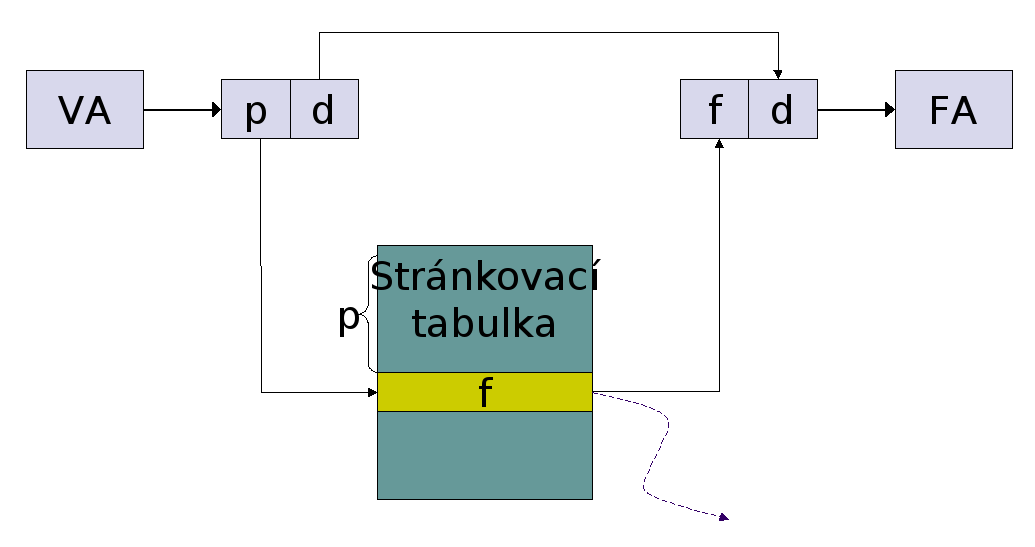
\includegraphics[width=10cm]{informatika/operacne_systemy_a_hw/obrazky/strankovani1.png}\end{center}
	\item umožnuje \emph{oddělené VAP} i \emph{sdílenou paměť} - mapování virtuální stránky 2 procesů na jednu fyzickou
	\item víceúrovňové stránkování (např. kvůli velikosti)
		\par \begin{center} 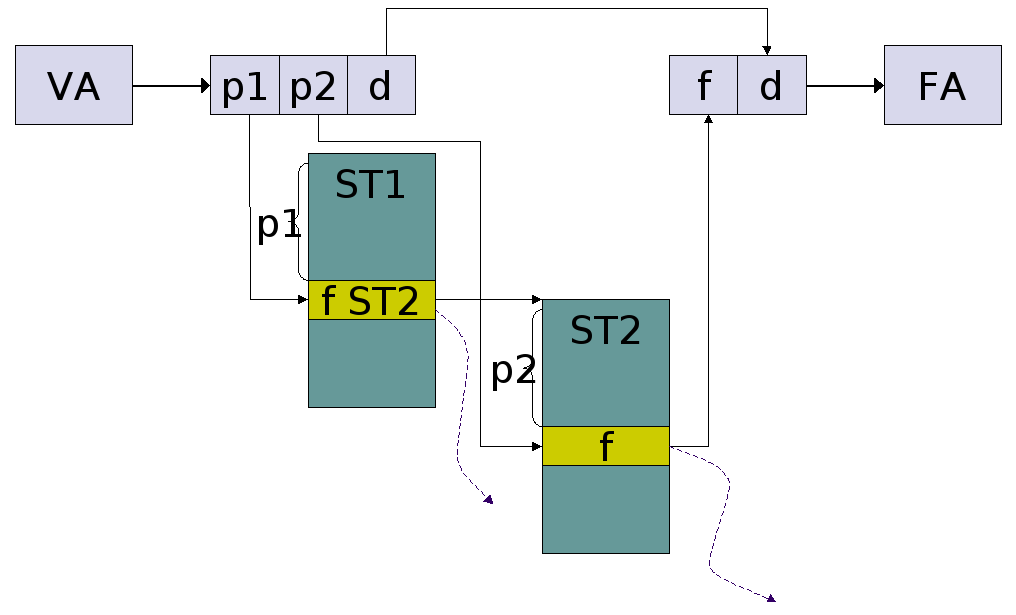
\includegraphics[width=10cm]{informatika/operacne_systemy_a_hw/obrazky/strankovani2.png} \end{center}
	\item TLB (Translation Lookaside Buffer) - asociativní paměť sloužící na rychlé vyhledání mapování virtuální stránky na fyzickou, využívá lokalitu chování programů
		\par \begin{center} 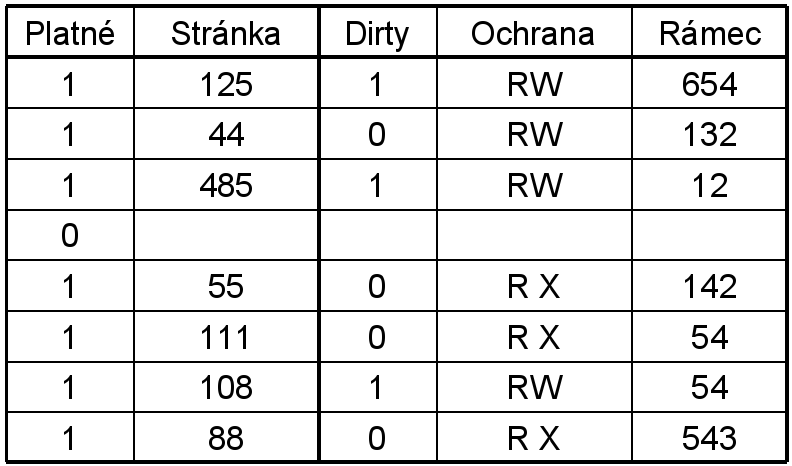
\includegraphics[width=6cm]{informatika/operacne_systemy_a_hw/obrazky/strankovani-tlb.png} \end{center} 
		\par ...nulaúrovňové stránkování - používá pouze TLB, řízeno také OS (oblíbené u 64-bitových CPU - UltraSPARC III)
	\item inverzní stránkování (např. když FAP je menší než VAP, 64-bitové CPU - IA-64)
		\par \begin{center} 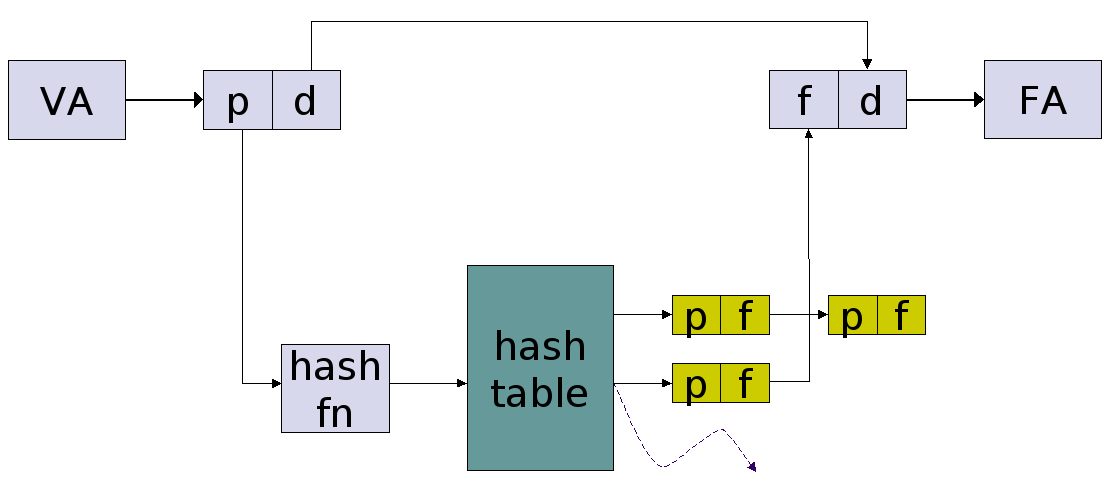
\includegraphics[width=10cm]{informatika/operacne_systemy_a_hw/obrazky/strankovani-inv.png} \end{center} 
\end{pitemize}

Akce vykonávané při výpadku stránky:
\begin{pitemize}
	\item výjimka procesoru
	\item uložit stav CPU (kontext)
	\item zjistit VA
	\item kontrola platnosti adresy a práv
	\item nalezení volného rámce
	\item zrušit mapování na nalezený rámec
	\item pokud je vyhazovaný rámec vyhazován, spustit ukládání na disk
	\item načíst z disku požadovanou stránku do rámce
	\item zavést mapování
	\item obnovit kontext
\end{pitemize}


Při implementaci stránkování je nutno brat v úvahu: 
\begin{pitemize}
    \item \emph{znovuspuštění instrukce} --- je potřeba aby procesor po výpadku zkusil přístup do paměti znova. dnes umí všechny CPU, např. 68xxx - problémy (přerušení v půlce instrukce) 
    \item \emph{sdílení stránek} --- jednomu rámci odp. víc stránek $\rightarrow$ pokud s ním něco dělám, týká se to všech stránek!  musím vše ost. odmapovat. musím si pamatovat mapování pro každý rámec - obrácené tabulky. 
    \item \emph{odstranění položky z TLB při rušení mapování} --- nestačí změnit tabulky, musí se vyhodit i z TLB (kde to může, ale nemusí být). problém - u multiprocesorů má každá CPU vlastní TLB, tabulky jsou sdílené $\rightarrow$ CPU při rušení mapování musí poslat interrupt s rozkazem ke smazání všem (i sobě), počkat na potvrzení akce od všech.
\end{pitemize}

\subsubsection*{Algoritmy pro výměnu stránek}
\begin{pitemize}
	\item \textbf{Optimální stránka} (v okamžiku výpadku stránky vybírám stránku, na níž se přistoupí za největší počet instrukcí) - nelze implementovat
	\item \textbf{NRU} (Not Recently Used) - každá stránka má příznaky Accessed a Dirty (typicky implementovatelné v HW, možno simulovat SW); jednou za čas se smažou všechna A; při výpadku rozdělím stránky podle A,D a vyberu stránku z nejnižší neprázdné třídy:
		\par \begin{center}
		\begin{tabular}{|c|c|c|}
			\hline 
			  & A & D \\
			\hline
			0 & 0 & 0 \\
			\hline
			1 & 0 & 1 \\
			\hline
			2 & 1 & 0 \\
			\hline
			3 & 1 & 1 \\
			\hline
		\end{tabular}
		\end{center}
	\item \textbf{FIFO} (vykazuje anomálie - Belady (zvětšení počtu výpadků stránky, když zvýšíme počet stránek v paměti)), druhá šance (úprava FIFO; pokud A=1, zařadím na konec FIFO... nevykazuje anomálie)
	\item \textbf{Hodiny} - modifikace druhé šance: kruhový zoznam stránek + iterátor na ukazující na nejstarší stránku v zoznamu. Při výpadku (a neexistenci volého rámce) se zjistí, jestli má *iterator nastavený příznak Accessed. Jestli ne, tato stránka bude nahrazena - v opačném případě se Accessed příznak zruší a iterator++. Toto se opakuje, dokud nedojde k výměně\dots
	\item \textbf{LRU} (Least Recently Used) - často používané stránky v posledním krátkém časovém úšeku budou znovu použity, čítač použití stránek, možné implementovat v HW
	\item \textbf{NFU} (Not Frequently Used) - SW simulace LRU, SW čítač ke každé stránce; jednou za čas projdu všechna A a přičtu je k odpovídajícím čítačům; vybírám stránku s nejnižším čítačem; nezapomíná - je možná modifikace se stárnutím čítače
\end{pitemize}

\subsubsection*{Segmentace}
dnes pouze Intel IA-32, dvojrozměrný VAP
\begin{pitemize}
	\item rozdělení programu na segmenty (napr. podle částí s různými vlastnostmi - kód, data, zásobníky\dots), různé délky segmentů, ktoré můžou měnit svoji délku za běhu
	\item VAP dvourozměrný (segment, offset), FAP jednorozměrný (vyzerá jako při spojitém pridělování paměti)
	\item segmentová převodní tabulka (VA se skládá ze dvou častí S:D, v tabulce se najde adresa segmentu S\dots k této adrese se poté přičte D, co je umístnění adresy v FA), příznak existence mapování
	\item při výpadku je nutné měnit celý segment (ty mohou být velké), je možné segmenty sesypat - ale nelze mít segment větší než FAP
\end{pitemize}

Segmentaci je možné kombinovat se stránkováním (odstraňuje nevýhody segmentace, neprovádí se výpadky segmentů):
\par \begin{center}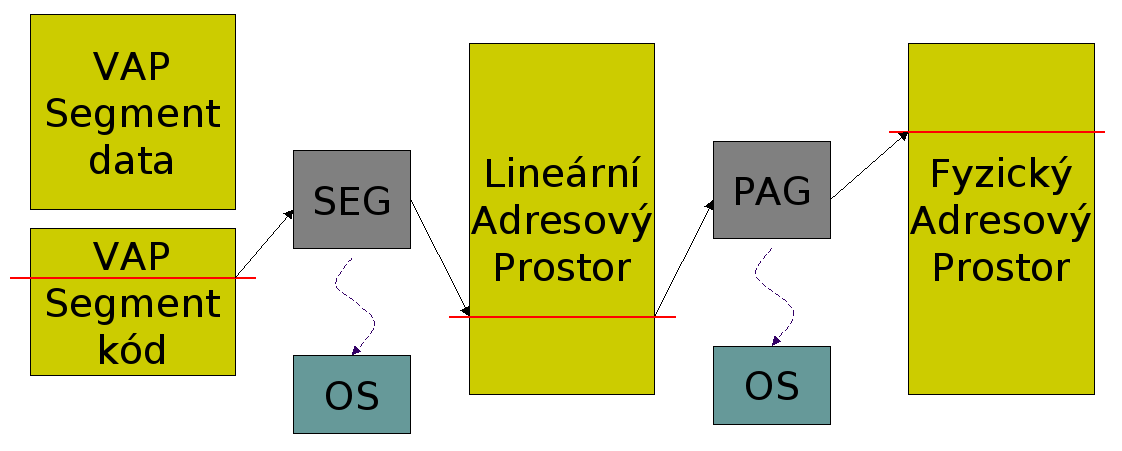
\includegraphics[width=12cm]{informatika/operacne_systemy_a_hw/obrazky/segmentace-a-strankovani.png}\end{center}

\subsection{Systémy souborů, adresářové struktury}

\begin{definiceN}{soubor}
  \emph{Soubor} je pojmenovaná množina souvisejících informací, která leží v
  pomocné paměti (na disku).\\
  \emph{Soubor} je abstrakce, která umožňuje uložit informaci na disk a později ji
  přečíst. Abstrakce odstiňuje uživatele od podrobností práce s disky.
\end{definiceN}

\begin{obecne}{Soubory}
  \begin{pitemize}
    \item pojmenování souboru (umožňuje uživateli přístup k jeho datům;
    přesná pravidla pojmenování určuje OS - malá vs. velká písmenka,
    speciální znaky, délka jména, přípony a jejich význam)
    \item atributy souborů (opět určuje OS) - jméno, typ, umístění, velikost, ochrana, časy, vlastník, \dots
    \item struktura souborů - sekvence bajtů / sekvence záznamů / strom
    \item typy souborů - běžné soubory, adresáře (systémové soubory vytvářející strukturu souborového systému), speciální soubory (znakové/blokové, soft linky)
    \item přístup 
    \begin{pitemize}
      \item \textbf{sekvenční}~-- pohyb pouze vpřed, OS může přednačítat
      \item \textbf{náhodný}~-- možno měnit aktuální pozici
      \item \textbf{paměťově mapované soubory}~-- pojmenovaná virtuální paměť,
      práce se souborem instrukcemi pro práci s pamětí, ušetří se kopírování
      pamětí; mají i problémy (přesná velikost souboru, zvětšování souboru,
      velikost souborů)
    \end{pitemize}
    \item volné místo na disku - bitmapa / spojový seznam volných bloků 
  \end{pitemize}
\end{obecne}

\begin{obecne}{Uložení souborů}
  Soubory se ukládají na disk po blocích
  \begin{pitemize}
    \item souvislá alokace - souvislý sled bloků
    \item spojovaná alokace - blok odkazuje na další
    \item indexová alokace - inode (UNIX) 
  \end{pitemize}
\end{obecne}

\begin{obecne}{Adresáře}
  \begin{pitemize}
    \item zvláštní typ souboru
    \item operace nad adresáři - hledání souboru / vypsání adresáře /
    přejmenování, vytvoření, smazání souboru 
    \item kořen, aktuální adresář, absolutní/relativní cesta
    \item hierarchická struktura 
    \begin{pitemize}
      \item \emph{strom}~-- jednoznačné pojmenování (cesta)
      \item \emph{DAG}~-- víceznačné pojmenování, ale nejsou cykly
      \item \emph{obecný graf}~-- cykly vytváří problém při prohledávání
    \end{pitemize}
    \item implementace adresářů - záznamy pevné velikosti, spojový seznam, B-stromy 
  \end{pitemize}
\end{obecne}

\begin{obecne}{Co musí filesystém umět?}
musí splňovat 3 věci: \emph{správu souborů} (kde jsou, jak velké), \emph{správu adresářů} (převod jméno $\leftrightarrow$ id) (někdy to dělá jiný prostředek, dnes větš. umí FS sám), \emph{správu volného místa}. někdy mohou být i další (odolnost proti výpadkům) 

Velikost bloků -- blok = nejmenší jednotka pro práci s diskem; disk pracuje s min. 1 sektorem (typicky 512 B) - někdy by pak bylo moc bloků $\rightarrow$ OS sdruží několik sektorů lineáně vedle sebe = 1 blok. velikost: velké = rychlejší práce, ale vnitřní fragmentace (průměrný soubor má cca pár KB), malé = malá vnitřní fragmentace, větší režie na info o volném místě/ umístění souboru (zabírá víc bloků!), navíc fragmentace souborů $\rightarrow$ zpomalení. dnes má blok cca 2-4KB.
\end{obecne}

\begin{obecne}{Linky}
  \begin{pitemize}
    \item \textbf{Hard link}~-- Na jedna data souboru se odkazuje z různých položek v adresářích
    \item \textbf{Soft link}~-- Speciální soubor, který obsahuje jméno souboru
  \end{pitemize}
\end{obecne}

\begin{priklady}
  \begin{pitemize}
    \item FAT -- \url{http://en.wikipedia.org/wiki/File\_Allocation\_Table}
    \item NTFS~-- charakteristika, MFT (Master File Table), run list\\\url{http://www.digit-life.com/articles/ntfs/}\\\url{http://www.pcguide.com/ref/hdd/file/ntfs/archSector-c.html}
    \item ext2/ext3~-- struktura, inode, žurnál\\\url{http://www.science.unitn.it/~fiorella/guidelinux/tlk/node95.html}\\\url{http://www.linux-security.cn/ebooks/ulk3-html/0596005652/understandlk-CHP-18.html}
  \end{pitemize}
\end{priklady}

\begin{obecne}{Plánování pohybu hlav disků}
  \begin{pitemize}
    \item FCFS (First-Come, First-Served) - žádné plánování, fronta požadavků, jeden za druhým
    \item SSTF (Shortest Seek Time First) - krajní žádosti mohou "hladovět"
    \item LOOK (výtah), C-LOOK (circular LOOK) - pohyb jen jedním směrem, na konci otočka 
  \end{pitemize}
\end{obecne}

\begin{obecne}{RAID (Redundant Array of Inexpensive Disks)}
  \begin{pitemize}
    \item JBOD (Just a Bunch of Disks)
    \item RAID 0~-- striping, žádná redundance
    \item RAID 1~-- mirroring, redundance
    \item RAID 0+1~-- mirroring a striping
    \item RAID 2~-- 7-bitový paritní Hammingův kód
    \item RAID 3~-- 1 paritní disk, po bitech na disky
    \item RAID 4~-- 1 paritní disk a striping
    \item RAID 5~-- distribuovaná parita a striping
    \item RAID 6~-- distribuovaná parita -- dvojitá P+Q, striping 
  \end{pitemize}
\end{obecne}

\subsection{Bezpečnost, autentifikace, autorizace, přístupová práva}

\begin{definice}
  \begin{pitemize}
    \item \textbf{Ochrana}~-- s prostředky OS mohou pracovat pouze autorizované procesy
    \item \textbf{Autorizace}~-- zjištění oprávněnosti požadavku
    \item \textbf{Bezpečnost}~-- zabraňuje neautorizovaný přístup do systému
    \item \textbf{Právo}~-- povolení/zakázání vykonávat nějakou operaci
    \item \textbf{Doména ochrany}~-- množina párů (objekt:práva)
    \begin{pitemize}
      \item \textbf{ACL (Access Control List)}~-- ke každému objektu seznam práv pro uživatele/skupiny
      \item \textbf{C-list (Capability List)}~-- ke každému uživateli/skupině seznam práv pro objekty
    \end{pitemize}
  \end{pitemize}
\end{definice}

\begin{obecne}{Autentifikace}
  Identifikace něčím, co uživatel ví, má nebo je. 
  \begin{pitemize}
    \item \textbf{Hesla}
    \begin{pitemize}
      \item slovníkový útok (80--90\% hesel je jednoduchých), hrubá síla
      \item vynucování délky a složitosti hesla
    \end{pitemize}
    \item \textbf{Model otázka/odpověď}
    \item \textbf{Fyzický objekt}~-- smartcards, USB klíče
    \item \textbf{Biometrika}~-- otisky prstů, rohovka, hlas
  \end{pitemize}
\end{obecne}

TODO: autorizace, přístupová práva

\subsection{Druhy útoků a obrana proti nim}

\subsubsection*{Vnitřní útoky}
\begin{pitemize}
  \item \textbf{Trojský kůň}~-- zdánlivě neškodný program obsahuje \uv{zlý} kód
  \item \textbf{Login spoofing}~-- falešná \uv{logovací} obrazovka
  \item \textbf{Logická bomba}~-- zaměstnanec vpraví kus kódu do systému, který
  musí být pravidelně informován o tom, že zaměstnanec je stále zaměstnancem
  \item \textbf{Zadní dvířka (trap door, back door)}~-- kód při nějaké podmínce
  přeskočí normální kontroly
  \item \textbf{Přetečení vyrovnávací paměti (buffer overflow)}
  \begin{pitemize}
    \item ve velkém množství kódu nejsou dělány kontroly na přetečení polí pevné velikosti
    \item při přetečení se typicky přepíše část zásobníku a lze tam umístit adresu kódu i samotný kód, který se vykoná při návratu z funkce
  \end{pitemize}
\end{pitemize}

\subsubsection*{Vnější útoky}
\begin{pitemize}
  \item \textbf{Virus}~-- vytvoří se nakažený \uv{žádaný} soubor
  \item \textbf{Internetový červ (worm)}~-- samoreplikující se program (červ),
  využívá nějaké chyby systému 
  \item \textbf{Mobilní kód}~-- applety, agenti\dots
\end{pitemize}

\subsubsection*{Útočníci}
Útočníkem může být buď náhodný uživatel, vnitřní pracovník, zločinec (zvenčí) nebo špion (vojenský, komerční). Cíle útoků jsou na důvěrnost -- zjištění obsahu, nebo celistvost -- změna obsahu, případně dostupnost služby -- Denial of service. Ke ztrátě dat může dojít i v důsledku chyby hardware, software, lidské chyby nebo Božího zásahu.

\subsubsection*{Obrana}
jsou to spíš banality, ale nic víc po nás nechtějí???
\begin{pitemize}
    \item proti trojanům, backdoorům, logical bomb -- omezení přístupových práv, metoda \uv{least privilege}
    \item proti login-spoofu -- \uv{secure attention key}, tj. takové to \uv{Začněte stisknutím Ctrl-Alt-Del}
    \item proti buffer overflow -- jedině patche
    \item proti virům -- antivirus ;-), anti-spyware 
    \item proti červům -- firewall, patche (útoky jsou většinou proti známým a opraveným chybám aplikací, proti druhému typu, tzv. \uv{zero-day attack} je jedinou obranou firewall)
    \item proti problémům s aplety a skripty -- sandboxing (běh v omezeném prostředí bez možnosti přístupu k počítači)
    \item proti všemu -- backupy ;-)
\end{pitemize}

\subsection{Kryptografické algoritmy a protokoly}

\begin{obecne}{Cíle kryptografie}
  \begin{pitemize}
    \item důvěrnost dat
    \item celistvost dat
    \item autentifikace~-- od koho jsou data
    \item nepopiratelnost~-- když jednou něco potvrdím, nemohu to popřít.
  \end{pitemize}
\end{obecne}

\begin{definiceN}{Kryptografický systém}
 \textbf{ Kryptografický systém} obsahuje:
  \begin{pitemize}
    \item prostor zpráv~-- \emph{plaintext},
    \item prostor šifrovaných zpráv~-- \emph{ciphertext},
    \item prostory šifrovacích a dešifrovacích \emph{klíčů},
    \item efektivní algoritmus pro \emph{generování klíčů},
    \item efektivní algoritmus pro \emph{šifrování},
    \item efektivní algoritmus pro \emph{dešifrování}.
  \end{pitemize}
\end{definiceN}

\begin{definiceN}{označení}
  $C$~-- šifra, $P$~-- otevřený text, $K$~-- klíč,\\
  $\mathbf{E}$~-- šifrovací algoritmus, $\mathbf{D}$~-- dešifrovací algoritmus.\\[3mm]
  \emph{Šifrování:} $C = \mathbf{E}(P)$, resp. $C = \mathbf{E}(K, P)$\\
  \emph{Dešifrování:} $P = \mathbf{D}(C)$, resp. $P = \mathbf{D}(K, C)$\\
\end{definiceN}


\begin{obecne}{Kerchoffovy principy dobrého krypt. systému}
\begin{pitemize}
    \item E a D neobs. tajnou část
    \item E distribuuje rozumné zprávy rovnoměrně po C
    \item se správným klíčem jsou E \& D efektivní
    \item bez správného klíče je dešifrování minimáně NP-úplné. 
\end{pitemize}
\end{obecne}

\begin{obecne}{dělení kryptografických systémů}
\begin{pitemize}
    \item symetrické krypt. systémy : $k = k'$
    \item asymetrické : $k \neq k'$ ( veřejný a tajný klíč ). 
\end{pitemize}
\end{obecne}

\begin{obecne}{Model útočníka podle Doleva a Yao}
\begin{pitemize}
    \item může získat jakokoliv zprávu jdoucí po síti, může zahájit komunikaci s jiným uživatelem, může se stát příjemcem zpráv od kohokoliv, může zasílat zprávy komukoliv \& vydávat se za jiného uživatele, 
    \item nemůže uhádnout náh. číslo z dost velké množiny, bez klíče nemůže dešifrovat zprávu \& nemůže vytvořit platnou šifrovanou zprávu (vzhledem k šifr. alg.).
\end{pitemize}
\end{obecne}

\subsubsection*{Kryptografické protokoly}

\begin{pitemize}
   \item \textbf{Arbitrované protokoly}~-- rozhodčí dělá skoro všechno.
   \item \textbf{Rozhodované protokoly}~-- rozhodčí je dobrý jenom při sporu aby rozhodl.
   \item \textbf{Samozabezpečovací protokoly}~-- není žádná třetí strana.
\end{pitemize}

\begin{obecne}{Anonymní platby}
  Problém kreditních karet spočívá v sledovatelnosti toku peněz. Hledáme protokol
  pro tvorbu autentizovaných ale nesledovatelných zpráv.
\end{obecne}

\begin{obecne}{Časové známky}
  Nejjednodušší metodou je zasílat kopie zpráv důvěryhodnému arbitrovi, problémy s
  množstvím uchovávaných dat lze vyřešit použitím hašovacích funkcí.

  Používají se spojené (linked) aby odesílatel spolu s arbitrem nemohli podvádět.
  \begin{penumerate}
    \item Odesílatel $S$ zašle arbitrovi $A$ hashkod zprávy $H_n$.
    \item $A$ vrátí odesílateli 
    $T_n=S_K(n,S,H_n,Tm_n;Id_{n-1},H_{n-1},T_{n-1},H(Id_{n-1},H_{n-1},T_{n-1}))$
    kde $n$ je pořadí zprávy, $Tm_n$ čas podpisu zprávy, $Id_{n-1}\ldots$ jsou informace
    o předešlé zprávě, kterou arbitr vyřizoval.
    \item Po vyřízení následující zprávy arbitr zašle odesílateli identifikaci
    následujícího odesilatele
  \end{penumerate}
  Chce-li někdo ověřit časovou známku zprávy, kontaktuje odesilatele $Id_{n-1}$ a
  $Id_{n+1}$ a pomoci nich ověří platnost $T_n$
\end{obecne}

\begin{obecne}{Digitální podpisy}
  Musí být nefalšovatelné, autentické, neměnitelné, \uv{nerecyklovatelné}.
  \paragraph{Symetrické systémy:}
   Nechť odesílatel $S$ zasílá příjemci $R$ zprávu $M$
   \begin{penumerate}
      \item $S$ zašle arbitrovi $A$ zprávu $\mathbf{E}(M,K_S)$.
      \item Arbitr verifikuje odesílatele a příjemci $R$ zašle 
      $\mathbf{E}((M,S, \mathbf{E}(M,K_S)),K_R)$
      \item Příjemce uchová $M$ a $\mathbf{E}(M,K_S)$ pro účely případného dokazování přijetí.
   \end{penumerate}

   \paragraph{Asymetrické systémy:}
   Stačí provést $\mathbf{E}(\mathbf{D}(M,K_S),K_R)$

\end{obecne}

\begin{obecne}{Důkazy s nulovou znalostí}
  \begin{pitemize}
    \item dokazovatel nesmí podvádět - pokud důkaz nezná, jeho šance přesvedčit arbitra
    je mizivá
    \item ověřovatel nesmí podvádět - o důkazu smí zjistit jenom to, ze ho dokazovatel zná.
    V žádném případě nesmí být schopen důkaz zrekonstruovat a sám provést.
    \item ověřovatel se nesmí dozvědět nic, co by nebyl schopen zjistit bez pomoci 
    dokazovatele.
  \end{pitemize}
  Není-li splněna poslední podmínka mluvíme o \emph{důkazech s minimálním vyzrazením}.
  Jeden z možných důkazů je založen na problematice Hamiltonovských kružnic v grafu.
  \begin{penumerate}
    \item Nechť $A$ zná Hamiltonovskou kružnici v grafu $G$.
    \item $A$ provede náhodnou permutaci očíslování vrcholů $G$. Původní graf a vzniklý $H$ jsou izomorfní.
    \item Kopie grafu $H$ je zaslána entitě $B$.
    \item Ověřovatel $B$ položí dokazovateli $A$ jednu z následujících otázek
    \begin{penumerate}
	\item Dokázat, že $G$ a $H$ jsou izomorfní
	\item Ukázat Hamiltonovskou kružnici v grafu $H$
    \end{penumerate}
    \item Opakováním kroku 1. až 4. lze docílit potřebné jistoty. 
  \end{penumerate}
\end{obecne}

\begin{obecne}{Neurčitý obnos (Oblivious transfer)}
  Protokol umožňuje, aby si adresát vybral z několika nabízených možností aniž
  by odesílatel předem znal jeho volbu, možné doplnění o následnou vzájemnou
  kontrolu.
\end{obecne}

\begin{obecne}{Podepisování kontraktů (Contract signing)}
  V každém okamžiku musí být obě smluvní strany vázány stejně moc.
  Nejjednodušším řešením je arbitrovaný protokol, kde obě strany předají
  centrální autoritě své podepsané kopie a tato třetí strana zajistí výměnu po
  obdržení obou kopií.
\end{obecne}

\begin{obecne}{Elektronická potvrzovaná pošta (digital certified mail)}
  Chceme, aby adresát mohl přečíst naši zprávu až poté, co získáme potvrzení o
  tom, že ji obdržel (elektronický doporučený dopis).
\end{obecne}

\begin{obecne}{Bezpečné volby}
  \begin{pitemize}
    \item volit smí pouze oprávnění voliči,
    \item každý smí hlasovat nejvýše jednou,
    \item nikdo nesmí vědět, kdo jak volil,
    \item nikdo nesmí měnit volbu jiných,
    \item každý hlas musí být započítán.
  \end{pitemize}

  Nejjednodušší možnost je použít protokol se dvěmi centrálními autoritami.
  Používá registrační autoritu $RA$ provádějící registraci voličů a sčítací
  autoritu $SA$, která sčítá hlasovací lístky a zveřejňuje výsledky voleb.
  \begin{penumerate}
    \item Všichni voliči zašlou $RA$ žádost o validační číslo.
    \item $RA$ zašle každému voliči náhodně zvolené validační číslo $L$ a zároveň
    si poznamená kdo jaké číslo dostal.
    \item $RA$ zašle seznam validačních čísel $SA$.
    \item Kazdy z voličů si náhodně vybere svoje identifikační číslo $Id$ a $SA$
    zašle zprávu $(L, Id, v)$ kde v je jeho volba.
    \item $SA$ porovná $L$ se seznamem validačních čísel z kroku 3. Odpovídající
    číslo škrtne a voličovo $Id$ přidá do seznamu asociovaného s voleným kandidátem.
    \item Po skončení voleb $SA$ zveřejní výsledky a seznamy identifikačních čísel
    spojené se jmény kandidátů.
  \end{penumerate}
\end{obecne}

\begin{obecne}{Útoky na protokoly}
  \begin{pitemize}
    \item \emph{přehrání zpráv}~-- M odposlouchá všechny zprávy a pak totéž udělá sám
    \item \emph{muž uprostřed} (man-in-the-middle)
    \item \emph{paralelní spojení}~-- několik běhů protokolů prováděných současně pod
    řízením M
    \item \emph{odražení}~-- A zahájí komunikaci, M zachytí zprávu, upraví ji, aby
    nebyl poznat původní A a pošle ji zpět A
    \item \emph{prokládání}~-- Několik běhů protokolu prováděných současně pod
    řízením M, zprávy z jednoho se použijí u dalšího, atd.
    \item \emph{chyba typu}~-- Nedodržení přesného sémantického významu zprávy
    \item \emph{vypuštění jména}~-- Pokud v protokolu není poznat, kdo za to může
    \item \emph{chybné použití šifrovací služby}~-- Špatný algoritmus použitý na nevhodném místě
  \end{pitemize}
\end{obecne}

\subsubsection*{Kryptografické algoritmy}

\begin{definiceN}{Substitution-box~-- S-box}
  \begin{pitemize}
    \item krabička která z \emph{m} bitů vstupu dělá \emph{n} bitů výstupu.
    \item někdy je použita pevná tabulka. Např. u DES
    \item někdy je výstup s-boxu závislý na klíči. Např. u Blowfish, Twofish
    \item v blokových šifrách je to často s-box kdo zamlžuje vztah mezi plaintextem a šifrou.
    \item dost často na něm závisí jak je šifra napadnutelná $\Rightarrow$ musí
    se volit dost obezřetně
  \end{pitemize}
\end{definiceN}

\begin{obecne}{Symetrické}
  \begin{pitemize}
    \item vysoká datová propustnost
    \item klíče na obou koncích musí zůstat utajeny $\Rightarrow$ je třeba často
    měnit klíče
    \item potřeba ověřené TTP (Trusted Third Party)
  \end{pitemize}
\end{obecne}

\begin{obecne}{DES}
  Vyvinula firma IBM na zakázku NBS počátkem 70. let. Původní název DEA, v USA
  DEA1. Jako standard přijat 23. 11. 1976 Dodnes používán v komerční sféře, pro
  vojenské účely není certifikován ani pro ochranu neklasifikovaných informací.
  Patrně nejrozsáhleji používaný šifrovací algoritmus všech dob.

  Šifruje 64-bitové bloky otevřeného textu na 64-bitové výstupní bloky, délka
  klíče 64 bitů.

  \begin{figure}[!ht]
    \begin{center}
      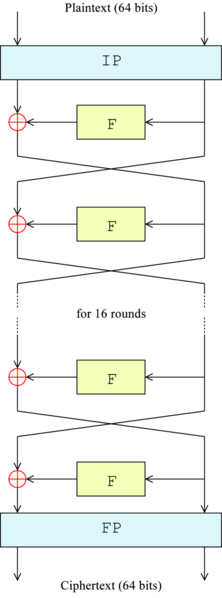
\includegraphics[scale=.7, angle=90]{informatika/algoritmy_a_ds/obrazky/DES-main-network.png}
      \caption{Struktura hlavní sítě algoritmu DES (zdroj: Wikipedie)}
    \end{center}
  \end{figure}

  \paragraph{Analýza:}
  \begin{pitemize}
    \item velká slabina je 64-bitový klíč (navíc efektivně pouze 56-bitový).
    Prolomen za méně než 24 hodin.
    \item úvodní permutace nemá prakticky žádný vliv
    \item existence slabých $(\mathbf{E}(K)=\mathbf{D}(K))$ a poloslabých
    $(\mathbf{E}(K_1)\mathbf{E}(K_2)=Id.)$ klíčů
    \item komplementárnost $C=\mathbf{E}(K,P)\Leftrightarrow\lnot C= \lnot
    \mathbf{E} (\lnot K,\lnot P)$
  \end{pitemize}
\end{obecne}

\begin{obecne}{Blowfish}
  \begin{pitemize}
    \item nástupce systému DES, 
    \item opět Feistelova šifra, délka bloku je 64 bitů, proměnná délka klíče až 448 bitů
    \item algoritmus provádí 16 cyklů nad vstupem délky 64-bitů
  \end{pitemize}
\end{obecne}

\begin{obecne}{IDEA}
  \begin{pitemize}
    \item z roku 1991, vyšel pod názvem IPES. 
    \item IDEA (International Data Encryption Algorithm)
    \item bloková šifra s délkou bloku 64-bitů a délkou klíče 128-bitu
    \item algoritmus je patentován 
    \item zajímavé je že pokud bychom algoritmus upravili tak, že bychom všechny řetězce
    se kterými pracuje zvětšili na dvojnásobek, tak dojde ke ztrátě bezpečnosti.
    \item algoritmus je považován za bezpečný.
  \end{pitemize}
\end{obecne}

\begin{obecne}{RC5}
  \begin{pitemize}
    \item z roku 1994 od R. Rivesta
    \item používá rotace závislé na datech.
    \item algoritmus umožňuje nastavit spoustu parametrů:
    \begin{pitemize}
      \item délka šifrovacího klíče (0\dots255 bytů)
      \item počet kol šifrovacího procesu (0\dots255)
      \item z hodnot 16, 32, 64, ale i vyšších lze zvolit délku slova, algoritmus
      zpracovává bloky o délce dvojnásobku slova
    \end{pitemize}
  \end{pitemize}

\end{obecne}

\begin{obecne}{Kryptosystém Rijndael}
  \begin{pitemize}
    \item produkční bloková šifra
    \item proměnná délka bloku~-- 16, 24 nebo 32 bajtů
    \item proměnná délka klíče~-- 128, 192 nebo 256 bitů
  \end{pitemize}

  \paragraph{Analýza:} Po rozsáhlé analýze nenalezena žádná slabina a tak
  zvolen jako nový standard AES.
\end{obecne}

\begin{obecne}{RC4}
  \begin{pitemize}
    \item proudová šifra od R. Rivesta
    \item jednoduchý a rychlý algoritmus 

    \paragraph{Analýza:} Zatím není známý žádný způsob útoku $\Rightarrow$
    algoritmus považován za bezpečný.
  \end{pitemize}
\end{obecne}

\begin{obecne}{FISH}
  \begin{pitemize}
    \item proudová šifra založena na Fibonacciho generátoru pseudonáhodných čísel.
    \item z fibonacciho generátoru se získá posloupnost a šifrovaní se provádí
    například XORováním této posloupnosti s \emph{P}
  \end{pitemize}
\end{obecne}

\begin{obecne}{Asymetrické}
  \begin{pitemize}
    \item šifry s asymetrickým klíčem~-- RSA, DSA (ElGammal)
    \item mnohem pomalejší
    \item není potřeba TTP
    \item pouze jeden klíč tajný, nemusí se měnit tak často
    \item o žádném schématu veřejného klíče nebylo dokázáno, že je bezpečné
  \end{pitemize}
\end{obecne}

\begin{obecne}{RSA}
  Kryptoschéma je založeno na Eulerově formuli: 
  $$a^{\varphi(n)} \equiv 1(mod\ n)$$ 
  kde $\varphi(n)$ je počet čísel z intervalu $1..n$ která jsou s $n$ nesoudělná.

  \paragraph{Šifrování:} Je třeba znát číslo $n$ a malé prvočíslo $e$. Otevřený
  text převedeme do posloupnosti modulo $n$. Každý blok $P_j$ zašifrujeme dle
  vzorce: $$C_j\equiv P_j^e\ (mod\ n)$$ Spojením výsledných bloků vznikne
  zašifrovaný text.

  \paragraph{Dešifrování:} Je třeba znát číslo $n$ a číslo $d$. Každý z bloků
  potom dešifrujeme takto: $$P_j\equiv C_j^d\ (mod\ n)$$ Pro dešifrovací klíč
  $d$ musí platit: $$ed\equiv 1\,(mod\ \varphi(n))$$ Prvočíslo $e$ nesmí dělit
  $\varphi(n)$. $d$ určíme z předchozího vztahu rozšířeným eukleidovým
  algoritmem.

  Veřejný klíč tvoří pár $(n, e)$, soukromý klíč pár $(n, d)$. Číslo $n$ musí být velmi
  velké a nesmí mít malé faktory. Pro reálné použití 100 až 200 bitů. Hranice bezpečnosti
  1024 bitů modulu $n$, rozumné 1500 bitů, lépe 2048 bitů.

  Není známa žádná metoda vedoucí k rozbití algoritmu RSA. 
\end{obecne}

\begin{obecne}{Merkle-Hellman kryptosystém}
  \begin{pitemize}
    \item založen na problému batohu
    \item plaintext je chápán jako posloupnost vah (řešení)
    \item ciphertext je výsledná hmotnost batohu
    \item pro superrostoucí posloupnost je problém řešitelný v lineárním čase
    \item superrostoucí posloupnost je součást soukromého klíče a tak
    dešifrování pomocí ní je zvládnutelné lineárně, kdežto bez ní je to NP-úplný
    problém
    \item systém byl prolomen! Není tedy považován za bezpečný. Útočník je
    schopen získat superrostoucí posloupnost a pomocí ní může dešifrovat
  \end{pitemize}
\end{obecne}

\begin{obecne}{Elgamal kryptosystém}
  Založen na obtížnosti výpočtu diskrétního logaritmu nad kruhem.

  Potřebujeme společný modul $q$ a číslo $g$ co nejvyššího řádu. Každý účastník si zvolí tajný
  klíč $y_i$ a vypočítá veřejný klíč $g^{y_i}$ mod $q$.
  \paragraph{Šifrování:} Nechť uživatel \emph{A} posílá zprávu \emph{P}
  uživateli \emph{B}. Náhodně
  vybere číslo $k$ a vypočítá: $$ g^k \mod q;\ P \otimes{(g^{y_b})}^k \mod q
  $$ obě čísla zašle \emph{B}.

  \paragraph{Dešifrování:} Uživatel \emph{B} vypočítá: $$ {(g^k)}^{y_b} \mod q$$
  a najde inverzní prvek. Z druhého čísla potom snadno získá \emph{P}.

  Systém je považován za bezpečný. Nevýhodou je nutnost generovat náhodné číslo
  $k$ a zdvojnásobení dat během šifrování.
\end{obecne}


\end{document}
